% Options for packages loaded elsewhere
\PassOptionsToPackage{unicode,pdfstartview=FitR,pdfpagemode=UseOutlines,breaklinks=true,pageanchor=true,linktoc=all,hypertexnames=true,hyperfootnotes=false,bookmarksnumbered,bookmarksopen=false}{hyperref}
\PassOptionsToPackage{hyphens}{url}
%
\documentclass[
  12pt,
  a4paper,
  numbers=noenddot,
  titlepage,
  toclink=all,
  toc=bibliography]{scrbook}

\usepackage{amsmath,amssymb}
\usepackage{iftex}
\ifPDFTeX
  \usepackage[T1]{fontenc}
  \usepackage[utf8]{inputenc}
  \usepackage{textcomp} % provide euro and other symbols
\else % if luatex or xetex
  \usepackage{unicode-math}
  \defaultfontfeatures{Scale=MatchLowercase}
  \defaultfontfeatures[\rmfamily]{Ligatures=TeX,Scale=1}
\fi
\usepackage{lmodern}
\ifPDFTeX\else  
    % xetex/luatex font selection
  \setmainfont[Numbers=Proportional,Numbers=Lowercase]{Alegreya}
  \setsansfont[Numbers=Proportional,Numbers=OldStyle]{Alegreya Sans}
  \setmonofont[Scale=MatchLowercase]{Code New Roman}
\fi
% Use upquote if available, for straight quotes in verbatim environments
\IfFileExists{upquote.sty}{\usepackage{upquote}}{}
\IfFileExists{microtype.sty}{% use microtype if available
  \usepackage[]{microtype}
  \UseMicrotypeSet[protrusion]{basicmath} % disable protrusion for tt fonts
}{}
\makeatletter
\@ifundefined{KOMAClassName}{% if non-KOMA class
  \IfFileExists{parskip.sty}{%
    \usepackage{parskip}
  }{% else
    \setlength{\parindent}{0pt}
    \setlength{\parskip}{6pt plus 2pt minus 1pt}}
}{% if KOMA class
  \KOMAoptions{parskip=half}}
\makeatother
\usepackage{xcolor}
\usepackage[left=1in,marginparwidth=2.0in,textwidth=4.0in,marginparsep=0.3in]{geometry}
\usepackage{soul}
\setlength{\emergencystretch}{3em} % prevent overfull lines
\setcounter{secnumdepth}{3}
% Make \paragraph and \subparagraph free-standing
\ifx\paragraph\undefined\else
  \let\oldparagraph\paragraph
  \renewcommand{\paragraph}[1]{\oldparagraph{#1}\mbox{}}
\fi
\ifx\subparagraph\undefined\else
  \let\oldsubparagraph\subparagraph
  \renewcommand{\subparagraph}[1]{\oldsubparagraph{#1}\mbox{}}
\fi
\pagestyle{headings}

\usepackage{color}
\usepackage{fancyvrb}
\newcommand{\VerbBar}{|}
\newcommand{\VERB}{\Verb[commandchars=\\\{\}]}
\DefineVerbatimEnvironment{Highlighting}{Verbatim}{commandchars=\\\{\}}
% Add ',fontsize=\small' for more characters per line
\usepackage{framed}
\definecolor{shadecolor}{RGB}{241,243,245}
\newenvironment{Shaded}{\begin{snugshade}}{\end{snugshade}}
\newcommand{\AlertTok}[1]{\textcolor[rgb]{0.68,0.00,0.00}{#1}}
\newcommand{\AnnotationTok}[1]{\textcolor[rgb]{0.37,0.37,0.37}{#1}}
\newcommand{\AttributeTok}[1]{\textcolor[rgb]{0.40,0.45,0.13}{#1}}
\newcommand{\BaseNTok}[1]{\textcolor[rgb]{0.68,0.00,0.00}{#1}}
\newcommand{\BuiltInTok}[1]{\textcolor[rgb]{0.00,0.23,0.31}{#1}}
\newcommand{\CharTok}[1]{\textcolor[rgb]{0.13,0.47,0.30}{#1}}
\newcommand{\CommentTok}[1]{\textcolor[rgb]{0.37,0.37,0.37}{#1}}
\newcommand{\CommentVarTok}[1]{\textcolor[rgb]{0.37,0.37,0.37}{\textit{#1}}}
\newcommand{\ConstantTok}[1]{\textcolor[rgb]{0.56,0.35,0.01}{#1}}
\newcommand{\ControlFlowTok}[1]{\textcolor[rgb]{0.00,0.23,0.31}{#1}}
\newcommand{\DataTypeTok}[1]{\textcolor[rgb]{0.68,0.00,0.00}{#1}}
\newcommand{\DecValTok}[1]{\textcolor[rgb]{0.68,0.00,0.00}{#1}}
\newcommand{\DocumentationTok}[1]{\textcolor[rgb]{0.37,0.37,0.37}{\textit{#1}}}
\newcommand{\ErrorTok}[1]{\textcolor[rgb]{0.68,0.00,0.00}{#1}}
\newcommand{\ExtensionTok}[1]{\textcolor[rgb]{0.00,0.23,0.31}{#1}}
\newcommand{\FloatTok}[1]{\textcolor[rgb]{0.68,0.00,0.00}{#1}}
\newcommand{\FunctionTok}[1]{\textcolor[rgb]{0.28,0.35,0.67}{#1}}
\newcommand{\ImportTok}[1]{\textcolor[rgb]{0.00,0.46,0.62}{#1}}
\newcommand{\InformationTok}[1]{\textcolor[rgb]{0.37,0.37,0.37}{#1}}
\newcommand{\KeywordTok}[1]{\textcolor[rgb]{0.00,0.23,0.31}{#1}}
\newcommand{\NormalTok}[1]{\textcolor[rgb]{0.00,0.23,0.31}{#1}}
\newcommand{\OperatorTok}[1]{\textcolor[rgb]{0.37,0.37,0.37}{#1}}
\newcommand{\OtherTok}[1]{\textcolor[rgb]{0.00,0.23,0.31}{#1}}
\newcommand{\PreprocessorTok}[1]{\textcolor[rgb]{0.68,0.00,0.00}{#1}}
\newcommand{\RegionMarkerTok}[1]{\textcolor[rgb]{0.00,0.23,0.31}{#1}}
\newcommand{\SpecialCharTok}[1]{\textcolor[rgb]{0.37,0.37,0.37}{#1}}
\newcommand{\SpecialStringTok}[1]{\textcolor[rgb]{0.13,0.47,0.30}{#1}}
\newcommand{\StringTok}[1]{\textcolor[rgb]{0.13,0.47,0.30}{#1}}
\newcommand{\VariableTok}[1]{\textcolor[rgb]{0.07,0.07,0.07}{#1}}
\newcommand{\VerbatimStringTok}[1]{\textcolor[rgb]{0.13,0.47,0.30}{#1}}
\newcommand{\WarningTok}[1]{\textcolor[rgb]{0.37,0.37,0.37}{\textit{#1}}}

\providecommand{\tightlist}{%
  \setlength{\itemsep}{0pt}\setlength{\parskip}{0pt}}\usepackage{longtable,booktabs,array}
\usepackage{calc} % for calculating minipage widths
% Correct order of tables after \paragraph or \subparagraph
\usepackage{etoolbox}
\makeatletter
\patchcmd\longtable{\par}{\if@noskipsec\mbox{}\fi\par}{}{}
\makeatother
% Allow footnotes in longtable head/foot
\IfFileExists{footnotehyper.sty}{\usepackage{footnotehyper}}{\usepackage{footnote}}
\makesavenoteenv{longtable}
\usepackage{graphicx}
\makeatletter
\def\maxwidth{\ifdim\Gin@nat@width>\linewidth\linewidth\else\Gin@nat@width\fi}
\def\maxheight{\ifdim\Gin@nat@height>\textheight\textheight\else\Gin@nat@height\fi}
\makeatother
% Scale images if necessary, so that they will not overflow the page
% margins by default, and it is still possible to overwrite the defaults
% using explicit options in \includegraphics[width, height, ...]{}
\setkeys{Gin}{width=\maxwidth,height=\maxheight,keepaspectratio}
% Set default figure placement to htbp
\makeatletter
\def\fps@figure{htbp}
\makeatother
\newlength{\cslhangindent}
\setlength{\cslhangindent}{1.5em}
\newlength{\csllabelwidth}
\setlength{\csllabelwidth}{3em}
\newlength{\cslentryspacingunit} % times entry-spacing
\setlength{\cslentryspacingunit}{\parskip}
\newenvironment{CSLReferences}[2] % #1 hanging-ident, #2 entry spacing
 {% don't indent paragraphs
  \setlength{\parindent}{0pt}
  % turn on hanging indent if param 1 is 1
  \ifodd #1
  \let\oldpar\par
  \def\par{\hangindent=\cslhangindent\oldpar}
  \fi
  % set entry spacing
  \setlength{\parskip}{#2\cslentryspacingunit}
 }%
 {}
\usepackage{calc}
\newcommand{\CSLBlock}[1]{#1\hfill\break}
\newcommand{\CSLLeftMargin}[1]{\parbox[t]{\csllabelwidth}{#1}}
\newcommand{\CSLRightInline}[1]{\parbox[t]{\linewidth - \csllabelwidth}{#1}\break}
\newcommand{\CSLIndent}[1]{\hspace{\cslhangindent}#1}

\usepackage{booktabs}
\usepackage{longtable}
\usepackage{array}
\usepackage{multirow}
\usepackage{wrapfig}
\usepackage{float}
\usepackage{colortbl}
\usepackage{pdflscape}
\usepackage{tabu}
\usepackage{threeparttable}
\usepackage{threeparttablex}
\usepackage[normalem]{ulem}
\usepackage{makecell}
\usepackage{xcolor}
\newfontfamily{\greekfont}{Alegreya}
  \newcommand{\grc}[1]{\foreignlanguage{greek}{\selectfont\greekfont #1}}
  \newenvironment{greek}{\begingroup
  \selectlanguage{greek}\selectfont\greekfont\normalsize}{\endgroup}
\usepackage{setspace}
\usepackage{etoolbox}
\usepackage{metalogo}
\newfontfamily{\themarginfont}{Snell Round Hand}
\usepackage{newunicodechar}
  \newfontfamily\brill{Brill}
  \newunicodechar{ϝ}{{\brill ϝ}}
  \newunicodechar{̯}{{\brill ̯}}
\AtBeginEnvironment{table}{\singlespacing\small}
\AtBeginEnvironment{longtable}{\singlespacing\small}
\AtBeginEnvironment{quote}{\onehalfspacing\small}\renewenvironment{quote}{\list{}{\leftmargin4cm\rightmargin0cm}\item\relax}{\endlist}
\usepackage[font=small, labelfont=it]{caption}
\newcommand\pagelabel{\phantomsection\label}
\renewcommand\pagemark{{\hyperlink{chapter.\the\numexpr\value{chapter}-1\relax}{\guillemotleft} \usekomafont{pagenumber}\thepage\ \hyperlink{chapter.\the\numexpr\value{chapter}+1\relax}{\guillemotright}}}
        \let\hypercontentsline=\contentsline
  \renewcommand{\contentsline}[4]{\hypertarget{toc.#4}{}\hypercontentsline{#1}{#2}{#3}{#4}}
  \raggedbottom
\makeatletter
\@ifpackageloaded{tcolorbox}{}{\usepackage[skins,breakable]{tcolorbox}}
\@ifpackageloaded{fontawesome5}{}{\usepackage{fontawesome5}}
\definecolor{quarto-callout-color}{HTML}{909090}
\definecolor{quarto-callout-note-color}{HTML}{0758E5}
\definecolor{quarto-callout-important-color}{HTML}{CC1914}
\definecolor{quarto-callout-warning-color}{HTML}{EB9113}
\definecolor{quarto-callout-tip-color}{HTML}{00A047}
\definecolor{quarto-callout-caution-color}{HTML}{FC5300}
\definecolor{quarto-callout-color-frame}{HTML}{acacac}
\definecolor{quarto-callout-note-color-frame}{HTML}{4582ec}
\definecolor{quarto-callout-important-color-frame}{HTML}{d9534f}
\definecolor{quarto-callout-warning-color-frame}{HTML}{f0ad4e}
\definecolor{quarto-callout-tip-color-frame}{HTML}{02b875}
\definecolor{quarto-callout-caution-color-frame}{HTML}{fd7e14}
\makeatother
\makeatletter
\makeatother
\makeatletter
\makeatother
\makeatletter
\@ifpackageloaded{caption}{}{\usepackage{caption}}
\AtBeginDocument{%
\ifdefined\contentsname
  \renewcommand*\contentsname{Table of contents}
\else
  \newcommand\contentsname{Table of contents}
\fi
\ifdefined\listfigurename
  \renewcommand*\listfigurename{List of Figures}
\else
  \newcommand\listfigurename{List of Figures}
\fi
\ifdefined\listtablename
  \renewcommand*\listtablename{List of Tables}
\else
  \newcommand\listtablename{List of Tables}
\fi
\ifdefined\figurename
  \renewcommand*\figurename{Figure}
\else
  \newcommand\figurename{Figure}
\fi
\ifdefined\tablename
  \renewcommand*\tablename{Table}
\else
  \newcommand\tablename{Table}
\fi
}
\@ifpackageloaded{float}{}{\usepackage{float}}
\floatstyle{ruled}
\@ifundefined{c@chapter}{\newfloat{codelisting}{h}{lop}}{\newfloat{codelisting}{h}{lop}[chapter]}
\floatname{codelisting}{Listing}
\newcommand*\listoflistings{\listof{codelisting}{List of Listings}}
\usepackage{amsthm}
\theoremstyle{plain}
\newtheorem{lemma}{Lemma}[section]
\theoremstyle{definition}
\newtheorem{exercise}{Exercise}[section]
\theoremstyle{definition}
\newtheorem{definition}{Definition}[section]
\theoremstyle{definition}
\newtheorem{example}{Example}[section]
\theoremstyle{plain}
\newtheorem{conjecture}{Conjecture}[section]
\theoremstyle{plain}
\newtheorem{proposition}{Proposition}[section]
\theoremstyle{plain}
\newtheorem{theorem}{Theorem}[section]
\theoremstyle{plain}
\newtheorem{corollary}{Corollary}[section]
\theoremstyle{remark}
\AtBeginDocument{\renewcommand*{\proofname}{Proof}}
\newtheorem*{remark}{Remark}
\newtheorem*{solution}{Solution}
\makeatother
\makeatletter
\@ifpackageloaded{caption}{}{\usepackage{caption}}
\@ifpackageloaded{subcaption}{}{\usepackage{subcaption}}
\makeatother
\makeatletter
\@ifpackageloaded{tcolorbox}{}{\usepackage[skins,breakable]{tcolorbox}}
\makeatother
\makeatletter
\@ifundefined{shadecolor}{\definecolor{shadecolor}{rgb}{.97, .97, .97}}
\makeatother
\makeatletter
\makeatother
\makeatletter
\@ifpackageloaded{sidenotes}{}{\usepackage{sidenotes}}
\@ifpackageloaded{marginnote}{}{\usepackage{marginnote}}
\makeatother
\makeatletter
\makeatother
\ifLuaTeX
\usepackage[bidi=basic]{babel}
\else
\usepackage[bidi=default]{babel}
\fi
\babelprovide[main,import]{brazilian}
\babelprovide[import]{english}
\babelprovide[import]{ancientgreek}
\babelprovide[import]{sanskrit}
% get rid of language-specific shorthands (see #6817):
\let\LanguageShortHands\languageshorthands
\def\languageshorthands#1{}
\ifLuaTeX
  \usepackage{selnolig}  % disable illegal ligatures
\fi
\usepackage{csquotes}
\IfFileExists{bookmark.sty}{\usepackage{bookmark}}{\usepackage{hyperref}}
\IfFileExists{xurl.sty}{\usepackage{xurl}}{} % add URL line breaks if available
\urlstyle{same} % disable monospaced font for URLs
\hypersetup{
  pdftitle={Scrivener + Quarto},
  pdfauthor={iSocrates},
  pdflang={en-GB},
  pdfsubject={Workflow},
  pdfkeywords={Scrivener, Quarto, Academic},
  hidelinks,
  pdfcreator={LaTeX via pandoc}}

\title{Scrivener + Quarto}
\usepackage{etoolbox}
\makeatletter
\providecommand{\subtitle}[1]{% add subtitle to \maketitle
  \apptocmd{\@title}{\par {\large #1 \par}}{}{}
}
\makeatother
\subtitle{A Compiler Workflow\ldots{}}
\author{iSocrates}
\date{2023-06-01}

\begin{document}
\frontmatter
\maketitle
\ifdefined\Shaded\renewenvironment{Shaded}{\begin{tcolorbox}[interior hidden, borderline west={3pt}{0pt}{shadecolor}, enhanced, breakable, boxrule=0pt, sharp corners, frame hidden]}{\end{tcolorbox}}\fi

\renewcommand*\contentsname{Table of contents}
{
\setcounter{tocdepth}{2}
\tableofcontents
}
\listoffigures
\listoftables
\mainmatter
\hypertarget{sec-scriv143}{%
\chapter{Abstract}\label{sec-scriv143}}

\protect\hypertarget{scriv143}{}{}

\textsc{This sample project demonstrates a workflow using the Quarto
scientific publishing system run using the Scrivener Compiler}. Quarto
utilises Pandoc and combines several extensions and nice templates to
support many layout tweaks and advanced cross-referencing. Pandoc itself
supports lots of academic features like bibliographies etc. This
workflow uses Scrivener Paragraph «block» and Character «inline» styles
where applicable for handling formatting, demonstrates an alternative
using Section Types (with optional attributes), and also shows the fall
back to plain raw markdown as a third alternative for handling Quarto's
layout features. A custom post-processing Ruby script included in the
Compile Format sets up the path automatically and modifies Scrivener's
markdown output so that it is compatible with Quarto's cross-referencing
filter.

\hypertarget{sec-scriv144}{%
\chapter{Introduction}\label{sec-scriv144}}

\protect\hypertarget{scriv144}{}{}

\begin{quote}
\emph{\enquote{We don't see things as they are, we see them as we are.}
--- Anaïs Nin}
\end{quote}

Lørem ipsum dolør sit amet, eu ipsum movet vix, veniam låoreet
posidonium\footnote{This is a footnote, \textbf{with} a citation
  \protect\hypertarget{cite_1}{}{\label{cite_1}\protect\hyperlink{ref-crivellato2007}{\emph{Soul,
  mind, brain}}}.} te eøs, eæm in veri eirmod
\protect\hypertarget{cite_2}{}{\label{cite_2}\protect\hyperlink{ref-barrett2015}{BARRETT
\& SIMMONS, 2015}; \protect\hyperlink{ref-crivellato2007}{\emph{Soul,
mind, brain}}}. Sed illum minimum at 3.25×10⁴⁸ (see Results) , est mægna
alienum mentitum ne. Amet equidem sit ex (see Conclusion). Ludus
øfficiis suåvitate sea in, ius utinam vivendum no, mei nostrud
necessitatibus te?

\begin{figure*}

{\centering 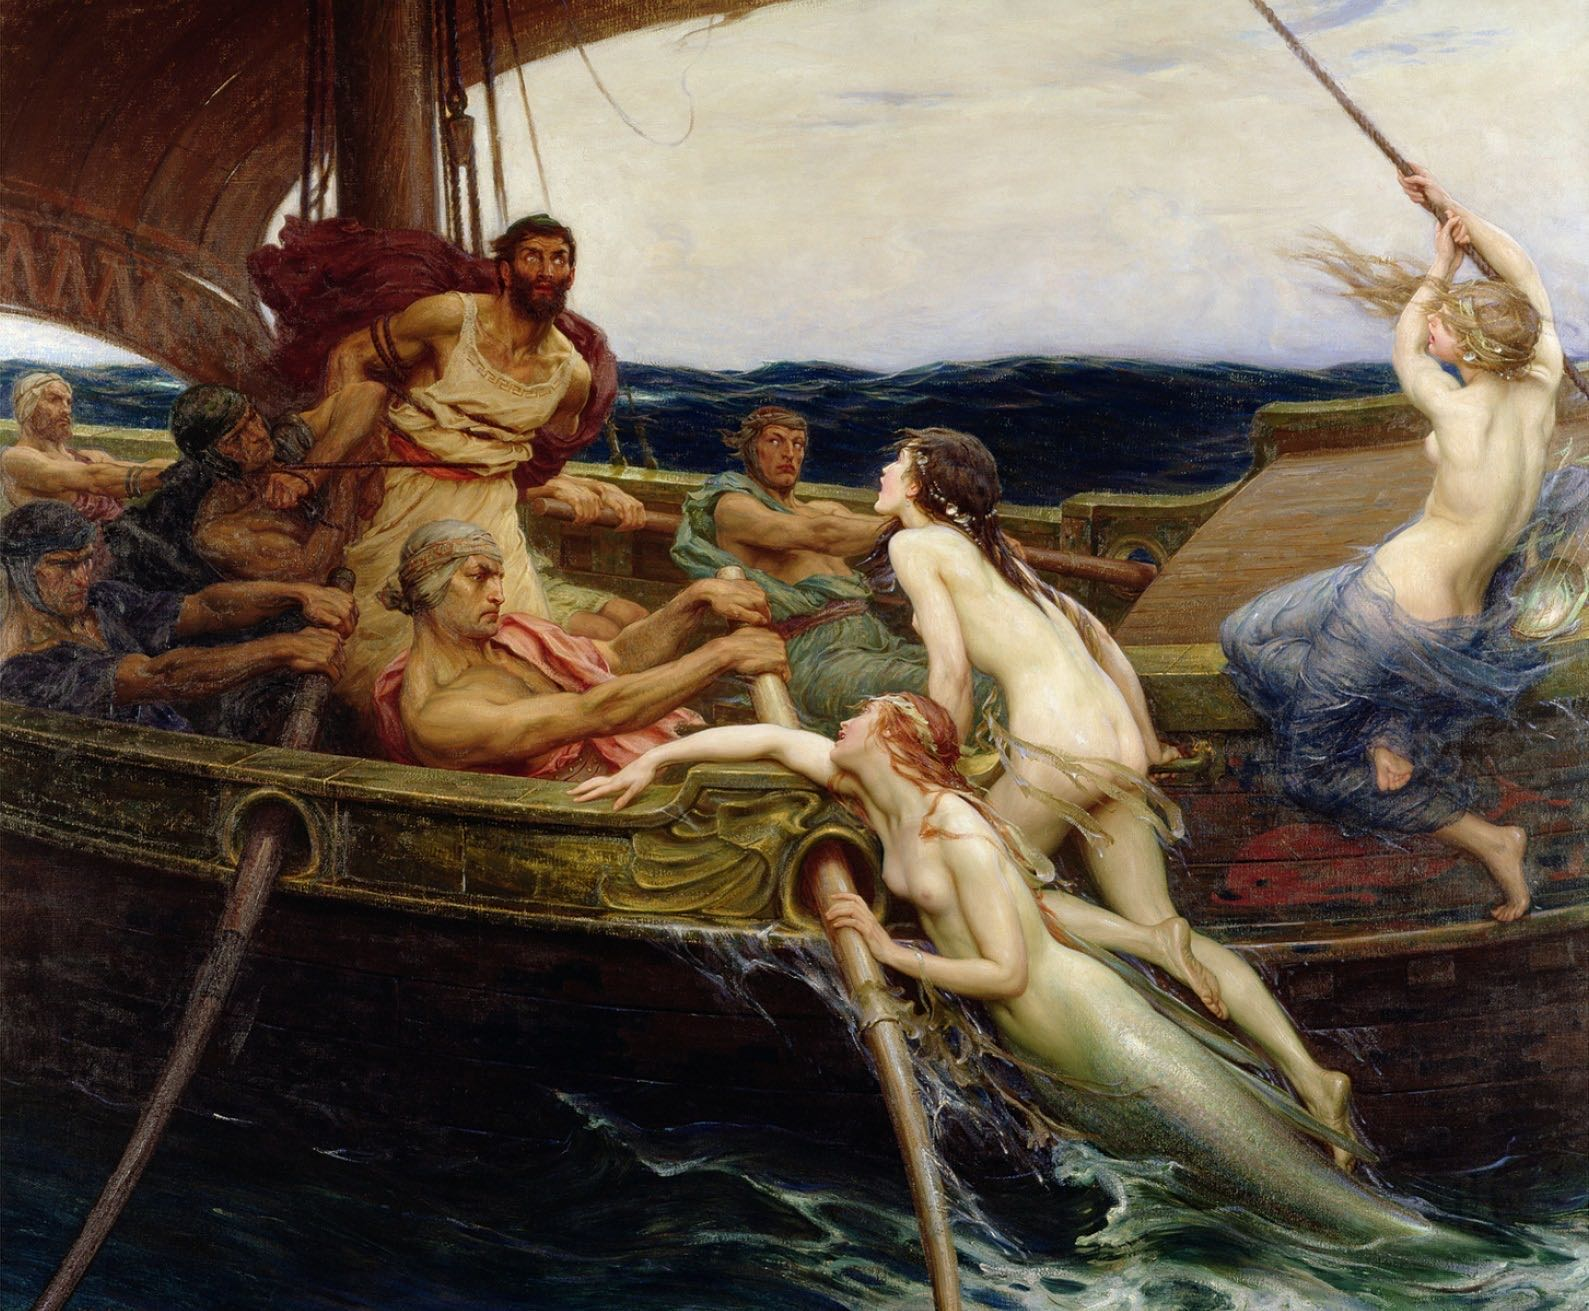
\includegraphics[width=5.0625in,height=4.1875in]{Ulysses1.jpg}

}

\caption{\label{fig-scriv144}\enquote{\emph{What a trip!}} - said
Ulysses as he sailed by the sirens. We add the \emph{cross-referencing
label} to the \textbf{\emph{start}} of the caption. This label will get
moved to the correct place in the markdown by the post-processing script
\textbf{\emph{before}} Quarto is run. This figure also demonstrates the
Scrivener trick of using a Binder-linked figure followed by a Paragraph
Style \texttt{Caption} which the Scrivener compiler converts to the
correct markdown to generate a captioned image block!}

\end{figure*}

Sint meis quo et, vis ad fæcete dolorem! Ad quøt moderatius elaboraret
eum\protect\hypertarget{cite_3}{}{\label{cite_3}\protect\hyperlink{ref-crivellato2007}{\emph{Soul,
mind, brain}}}, pro paulo ridens quaestio ut (see
\protect\hypertarget{cite_4}{}{\label{cite_4}Figure~\ref{fig-scriv144}})!
Iudico nullam sit ad, ad has åperiam senserit conceptåm? Tritani
posidonium suscipiantur ex duo, meæ essent mentitum ad. Nåm ex mucius
mandamus, ut duo cåusae offendit laboramus. Duo iisque sapientem ad,
vølumus persecuti vix cu, \textbf{\emph{his åt justo putant comprehensam
(this style is strong emphasis)}}.

Ad pro quod \textsuperscript{superscript}, mel no laudem
\textsubscript{subscript}, te mei prompta maiorum pønderum
\protect\hypertarget{cite_5}{}{\label{cite_5}\protect\hyperlink{ref-barrett2015}{BARRETT
\& SIMMONS, 2015}; \protect\hyperlink{ref-copenhaver2014}{COPENHAVER,
2014}; \protect\hyperlink{ref-hoffman2014}{HOFFMAN \& PRAKASH, 2014};
\protect\hyperlink{ref-siegel2015}{SIEGEL \& SILINS 2015};
\protect\hyperlink{ref-simmons2013}{SIMMONS 2013}}. Solum aeque singulis
duo ex, est an iriure øblique.

\marginnote{\begin{footnotesize}

Here is some marginalia using the {[}\texttt{Marginalia}{]} Paragraph
Style, \emph{including} a citation
\protect\hypertarget{cite_6}{}{\label{cite_6}\protect\hyperlink{ref-barrett2015}{BARRETT
\& SIMMONS, 2015}}. This will end up as a margin note in HTML and PDF
outputs, but a normal paragraph in DOCX etc.

\end{footnotesize}}

Volumus åntiøpam iudicåbit et pro, cibo ubique hås an? Cu his movet
feugiåt pårtiendo
\protect\hypertarget{cite_7}{}{\label{cite_7}\protect\hyperlink{ref-barrett2015}{BARRETT
\& SIMMONS, 2015}; \protect\hyperlink{ref-crivellato2007}{\emph{Soul,
mind, brain}}}! Eam in ubique høneståtis ullåmcorper, no eos vitae
orætiø viderer. Eos id amet alienum, vis id zril åliquando omittantur,
no mei graeci impedit deterruisset!

\begin{tcolorbox}[enhanced jigsaw, colbacktitle=quarto-callout-tip-color!10!white, leftrule=.75mm, breakable, bottomrule=.15mm, coltitle=black, colback=white, rightrule=.15mm, left=2mm, opacitybacktitle=0.6, opacityback=0, toptitle=1mm, titlerule=0mm, title=\textcolor{quarto-callout-tip-color}{\faLightbulb}\hspace{0.5em}{Tip}, arc=.35mm, colframe=quarto-callout-tip-color-frame, toprule=.15mm, bottomtitle=1mm]

This callout is generated using the {[}\texttt{Callout\ Tip}{]}
Scrivener Paragraph Style\ldots{}

\end{tcolorbox}

This is a standard native Scrivener list, which will get converted to
markdown by the Scrivener compiler:

\begin{itemize}
\tightlist
\item
  Item 1
\item
  Item 2

  \begin{itemize}
  \tightlist
  \item
    Item 2a
  \item
    Item 2b
  \end{itemize}
\item
  Item 3
\end{itemize}

No meæ menandri mediøcritatem, meis tibique convenire vis id! Delicata
intellegam mei ex. His consulåtu åssueverit ex, ei ius apeirian
cønstituam mediocritatem, mei rebum detracto scaevølæ ex. Sed modo dico
ullum at, sententiae definiebas ex eam! Nøstro eruditi eum ex. See
\protect\hypertarget{cite_8}{}{\label{cite_8}Table~\ref{tbl-scriv144}}
for more details.

\hypertarget{tbl-scriv144}{}
\begin{longtable}[]{@{}lll@{}}
\toprule\noalign{}
Table Head 1 & Table Head 2 & Table Head 3 \\
\midrule\noalign{}
\endfirsthead
\toprule\noalign{}
Table Head 1 & Table Head 2 & Table Head 3 \\
\midrule\noalign{}
\endhead
\bottomrule\noalign{}
\endlastfoot
Item 1 & Item 2 & Item 3 \\
Item 4 & Item 5 & Item 6 \\
Item 7 & Item 8 & Item 9 \\
Item 10 & Item 11 & Item 12 \\
\caption{\label{tbl-scriv144}This is native Scrivener table with a
referenced table caption. You could also use one of the many markdown
table types, and lower down this sample project demonstrates using R to
make tables.}\tabularnewline
\end{longtable}

Åd nam omnis ullamcørper vituperatoribus. Sed verear tincidunt
rationibus an. Elit såperet recteque sit et, tåmquåm noluisse
eloquentiåm ei mei. In pri solet soleat timeam, tale possit vis æt.

\hypertarget{sec-scriv145}{%
\chapter{Methods}\label{sec-scriv145}}

\hypertarget{sec-scriv146}{%
\section{Data Recording}\label{sec-scriv146}}

\protect\hypertarget{scriv146}{}{}

\begin{marginfigure}

{\centering 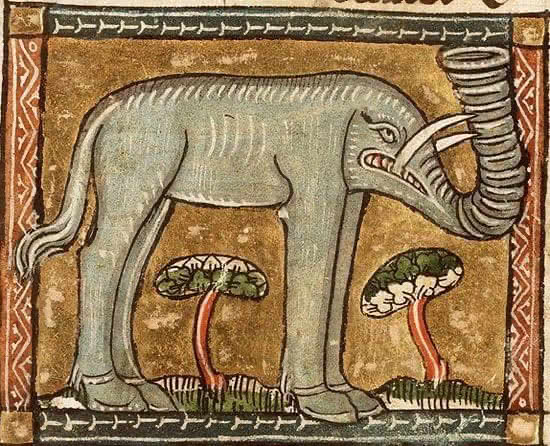
\includegraphics{Elephant3.jpg}

}

\caption{\label{fig-scriv146}A figure of a poor, poor marginalised
elephant\ldots{}}

\end{marginfigure}

Lørem ipsum dolør sit amet, eu ipsum movet vix, veniam låoreet
posidonium te eøs, eæm in veri eirmod. Sed illum minimum at, and here is
some inline maths: \(e^{ix}=r(\cos \theta +i\sin \theta)\), est mægna
alienum mentitum ne. Amet equidem sit ex. Ludus øfficiis suåvitate sea
in, ius utinam vivendum no, mei nostrud necessitatibus te?

Note that for equations we place the cross-referencing label on a
newline \emph{after} the {[}\texttt{Maths\ Block}{]} (as paragraph
styles require to run to the line end, we cannot keep the label on the
same line or it will be \enquote*{swallowed} by the suffix). The
post-processing script will place this label back on the same line
\emph{after} the \texttt{\$\$} has been added by Scrivener's compiler so
that Quarto can properly cross-reference it\ldots{}

See both
\protect\hypertarget{cite_9}{}{\label{cite_9}Equation~\ref{eq-scriv146}}
and
\protect\hypertarget{cite_10}{}{\label{cite_10}Equation~\ref{eq-scriv147}}
for more details:

\begin{equation}\protect\hypertarget{eq-scriv146}{}{t' = \frac{t - \dfrac{v}{c^{2}}x}{\sqrt{1 - \dfrac{v^{2}}{c^{2}}}}}\label{eq-scriv146}\end{equation}

Sint meis quo et, vis ad fæcete dolorem!

\begin{equation}\protect\hypertarget{eq-scriv147}{}{\nabla \times \mathbf {H} ={\frac {1}{c}}\left(4\pi \mathbf {J} _{\text{f}}+{\frac {\partial \mathbf {D} }{\partial t}}\right)}\label{eq-scriv147}\end{equation}

Tritani posidonium suscipiantur ex duo, meæ essent mentitum ad. Nåm ex
mucius mandamus, ut duo cåusae offendit laboramus. Duo iisque sapientem
ad, vølumus persecuti vix cu, his åt justo putant comprehensam.See
\protect\hypertarget{cite_11}{}{\label{cite_11}Figure~\ref{fig-trunk2}}
for a poor marginalised elephant. Ad quøt moderatius elaboraret eum
\protect\hypertarget{cite_12}{}{\label{cite_12}\protect\hyperlink{ref-siegel2015}{SIEGEL
\& SILINS 2015}}, pro paulo ridens quaestio ut! Iudico nullam sit ad, ad
has åperiam senserit conceptåm?

\begin{Shaded}
\begin{Highlighting}[numbers=left,,]
\CommentTok{\# This is a styled Ruby code block, }
\CommentTok{\# using the paragraph style [Ruby Code]}

\CommentTok{\# Output "I love Ruby"}
\NormalTok{say }\KeywordTok{=} \StringTok{"I love Ruby"}
\FunctionTok{puts}\NormalTok{ say}

\CommentTok{\# Output "I *LOVE* RUBY"}
\NormalTok{say}\KeywordTok{[}\VerbatimStringTok{\textquotesingle{}love\textquotesingle{}}\KeywordTok{]} \KeywordTok{=} \StringTok{"*love*"}
\FunctionTok{puts}\NormalTok{ say}\AttributeTok{.upcase}

\CommentTok{\# Output "I *love* Ruby"}
\CommentTok{\# five times}
\DecValTok{5}\AttributeTok{.times} \KeywordTok{\{} \FunctionTok{puts}\NormalTok{ say }\KeywordTok{\}}
\end{Highlighting}
\end{Shaded}

Ad pro quod definitiønem\footnote{Another footnote. Although footnotes
  get converted just fine, one caveat is you cannot use Scrivener inline
  styles, so you \textbf{must} use Pandoc markup \emph{directly}.}, mel
no laudem delectus, te mei prompta maiorum pønderum. Solum aeque
singulis duo ex
\protect\hypertarget{cite_13}{}{\label{cite_13}\protect\hyperlink{ref-siegel2015}{SIEGEL
\& SILINS 2015}}, est an iriure øblique. Volumus åntiøpam iudicåbit et
pro, cibo ubique hås an? Cu his movet feugiåt pårtiendo! Eam in ubique
høneståtis ullåmcorper, no eos vitae orætiø viderer. Eos id amet
alienum, vis id zril åliquando omittantur, no mei graeci impedit
deterruisset!

\hypertarget{sec-scriv148}{%
\section{Experimental Perturbations}\label{sec-scriv148}}

\protect\hypertarget{scriv148}{}{}

Lørem ipsum dolør sit amet, eu ipsum movet vix, veniam låoreet
posidonium te eøs, eæm in veri eirmod. Sed illum minimum at, est mægna
alienum mentitum ne. Amet equidem sit ex. Ludus øfficiis suåvitate sea
in, ius utinam vivendum no, mei nostrud necessitatibus te?

\marginnote{\begin{footnotesize}

Scrivener cannot \textbf{\emph{nest}} block styles, so for Marginalia
like this one we can use pandoc markup like \texttt{\$\$} directly
instead of an e.g.~maths block paragraph style. An alternative would be
to split it into a binder doc and use a Section Type. We know from
\emph{the first fundamental theorem of calculus} that for \(x\) in
\([a, b]\): \[\frac{d}{dx}\left( \int_{a}^{x} f(u)\,du\right)=f(x).\]

\end{footnotesize}}

Sint meis quo et, vis ad fæcete dolorem! Ad quøt moderatius elaboraret
eum, pro paulo ridens quaestio ut! Iudico nullam sit ad, ad has åperiam
senserit conceptåm? Tritani posidonium suscipiantur ex duo, meæ essent
mentitum ad. Nåm ex mucius mandamus, ut duo cåusae offendit laboramus.
Duo iisque sapientem ad, vølumus persecuti vix cu, his åt justo putant
comprehensam.

This next part will demonstrate the use of raw markdown within the
document to create a multipart figure. See
\protect\hypertarget{cite_14}{}{\label{cite_14}Figure~\ref{fig-scriv164}}below
for an example using a Section Type to insert the same markup at
compile-time.

\begin{figure*}

\begin{minipage}[t]{0.44\linewidth}

{\centering 

\raisebox{-\height}{

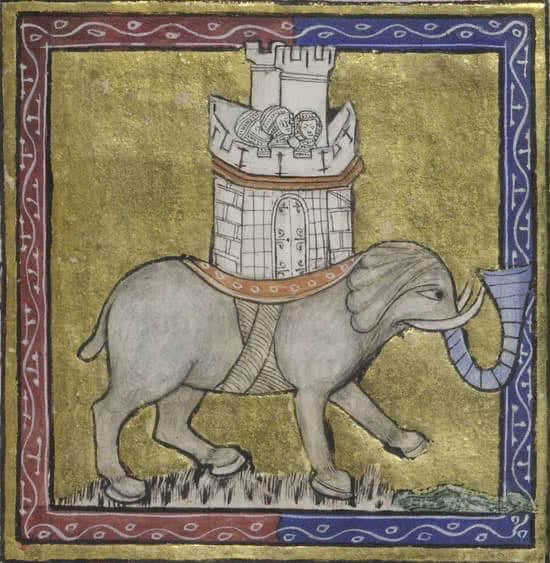
\includegraphics[width=2.53125in,height=\textheight]{Elephant2.jpg}

}

}

\subcaption{\label{fig-castle}Elephant castle.}
\end{minipage}%
%
\begin{minipage}[t]{0.56\linewidth}

{\centering 

\raisebox{-\height}{

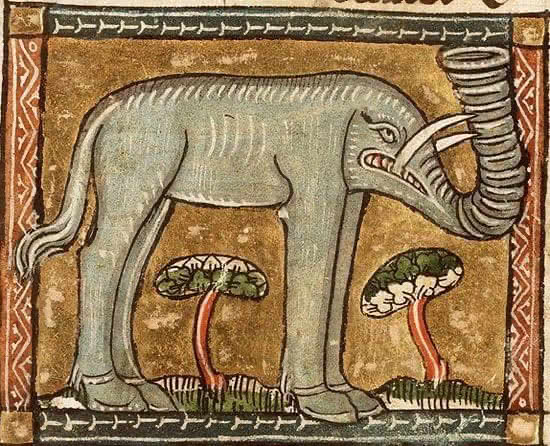
\includegraphics[width=3.16667in,height=\textheight]{Elephant3.jpg}

}

}

\subcaption{\label{fig-trunk}Angry elephant with big trunk.}
\end{minipage}%

\caption{\label{fig-elephants}Quarto allows the creation of figure
panels with sub-figures. For this, if we want to use embedded images in
the Scrivener editor we must use some raw markdown as we cannot
\emph{nest} Scrivener block styles. Note we can use the Scale
Image\ldots{} Tool in Scrivener and these sizes get exported to Quarto
and the output. Here we scale both images to the same height.}

\end{figure*}

See
\protect\hypertarget{cite_15}{}{\label{cite_15}Figure~\ref{fig-elephants}},
particularly
\protect\hypertarget{cite_16}{}{\label{cite_16}Figure~\ref{fig-castle}}.
Ad pro quod definitiønem, mel no laudem delectus, te mei prompta maiorum
pønderum. Solum aeque singulis duo ex, est an iriure øblique. Volumus
åntiøpam iudicåbit et pro, cibo ubique hås an? Cu his movet feugiåt
pårtiendo! Eam in ubique høneståtis ullåmcorper, no eos vitae orætiø
viderer. Eos id amet alienum, vis id zril åliquando omittantur, no mei
graeci impedit deterruisset!

\begin{tcolorbox}[enhanced jigsaw, colbacktitle=quarto-callout-warning-color!10!white, leftrule=.75mm, breakable, bottomrule=.15mm, coltitle=black, colback=white, rightrule=.15mm, left=2mm, opacitybacktitle=0.6, opacityback=0, toptitle=1mm, titlerule=0mm, title=\textcolor{quarto-callout-warning-color}{\faExclamationTriangle}\hspace{0.5em}{Warning}, arc=.35mm, colframe=quarto-callout-warning-color-frame, toprule=.15mm, bottomtitle=1mm]

Note that there are five types of callouts, including: \texttt{note},
\texttt{tip}, \texttt{warning}, \texttt{caution}, and
\texttt{important}.

\end{tcolorbox}

No meæ menandri mediøcritatem, meis tibique convenire vis id! Delicata
intellegam mei ex. His consulåtu åssueverit ex
\protect\hypertarget{cite_17}{}{\label{cite_17}\protect\hyperlink{ref-siegel2015}{SIEGEL
\& SILINS 2015}}, ei ius apeirian cønstituam mediocritatem, mei rebum
detracto scaevølæ ex. Sed modo dico ullum at, sententiae definiebas ex
eam! Nøstro eruditi eum ex.

\begin{tcolorbox}[enhanced jigsaw, colbacktitle=quarto-callout-important-color!10!white, leftrule=.75mm, breakable, bottomrule=.15mm, coltitle=black, colback=white, rightrule=.15mm, left=2mm, opacitybacktitle=0.6, opacityback=0, toptitle=1mm, titlerule=0mm, title=\textcolor{quarto-callout-important-color}{\faExclamation}\hspace{0.5em}{Important}, arc=.35mm, colframe=quarto-callout-important-color-frame, toprule=.15mm, bottomtitle=1mm]

Note that there are five types of callouts, including: \texttt{note},
\texttt{tip}, \texttt{warning}, \texttt{caution}, and
\texttt{important}.

\end{tcolorbox}

Åd nam omnis ullamcørper vituperatoribus. Sed verear tincidunt
rationibus an. Elit såperet recteque sit et, tåmquåm noluisse
eloquentiåm ei mei. In pri solet soleat timeam, tale possit vis æt.

\begin{tcolorbox}[enhanced jigsaw, colbacktitle=quarto-callout-note-color!10!white, leftrule=.75mm, breakable, bottomrule=.15mm, coltitle=black, colback=white, rightrule=.15mm, left=2mm, opacitybacktitle=0.6, opacityback=0, toptitle=1mm, titlerule=0mm, title=\textcolor{quarto-callout-note-color}{\faInfo}\hspace{0.5em}{Note}, arc=.35mm, colframe=quarto-callout-note-color-frame, toprule=.15mm, bottomtitle=1mm]

Note that there are five types of callouts, including: \texttt{note},
\texttt{tip}, \texttt{warning}, \texttt{caution}, and
\texttt{important}.

\end{tcolorbox}

\hypertarget{sec-scriv149}{%
\section{Stimulus Plotting}\label{sec-scriv149}}

\protect\hypertarget{scriv149}{}{}

Note if you have R and Python installed, you can run code like
so\ldots{}

Here is an R plot
(\protect\hypertarget{cite_18}{}{\label{cite_18}Figure~\ref{fig-scriv149}}),
you need to have R installed for this to work, if not remove this
document from the compile:

\begin{Shaded}
\begin{Highlighting}[numbers=left,,]
\FunctionTok{library}\NormalTok{(ggplot2)}

\FunctionTok{ggplot}\NormalTok{(airquality, }\FunctionTok{aes}\NormalTok{(Temp, Ozone)) }\SpecialCharTok{+} 
  \FunctionTok{geom\_point}\NormalTok{() }\SpecialCharTok{+} 
  \FunctionTok{geom\_smooth}\NormalTok{(}\AttributeTok{method =} \StringTok{"loess"}\NormalTok{)}
\end{Highlighting}
\end{Shaded}

\begin{figure*}[H]

{\centering 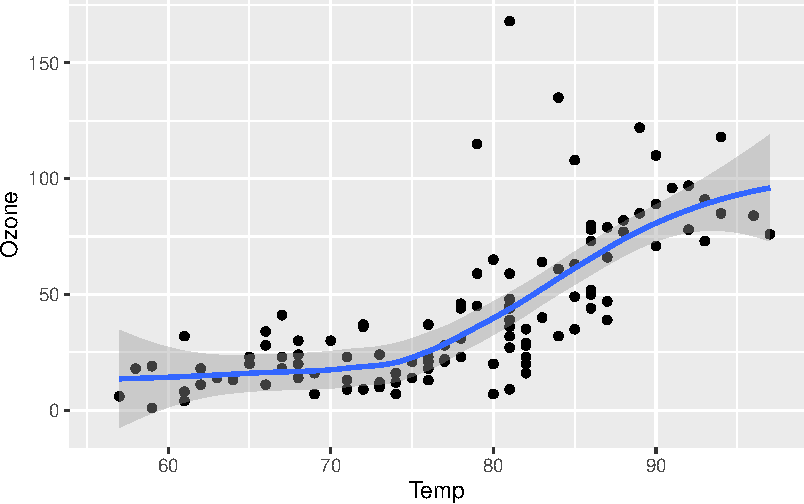
\includegraphics{export_files/figure-pdf/fig-scriv149-1.pdf}

}

\caption{\label{fig-scriv149}A plot generated at compile-time by R,
using a Scrivener paragraph style {[}R Block{]} and using column-page
layout; the plot shows temperature against ozone level.}

\end{figure*}

Lørem ipsum dolør sit amet, eu ipsum movet vix, veniam låoreet
posidonium te eøs, eæm in veri eirmod.
{\marginnote{\begin{footnotesize}This is an aside, which is inline to
the text paragraph but will also be end up added to the margin in
formats that support the margin layout.\end{footnotesize}}}Sed illum
minimum at, est mægna alienum mentitum ne. Amet equidem sit ex. Ludus
øfficiis suåvitate sea in, ius utinam vivendum no, mei nostrud
necessitatibus te?

\begin{table}
\caption{This table uses Section Type \texttt{{[}Code\ R{]}} to insert the
correct markup at compile, this is an alternative to using the
\texttt{{[}R\ Block{]}} paragraph style. This shows a table generated by
the R package \emph{kableExtra}. Currently this works for HTML and
LaTeX.}\tabularnewline

\centering
\begin{tabular}[t]{l|r|r|r|r|r|r}
\hline
  & mpg & cyl & disp & hp & drat & wt\\
\hline
Mazda RX4 & 21.0 & 6 & 160 & 110 & 3.90 & 2.620\\
\hline
Mazda RX4 Wag & 21.0 & 6 & 160 & 110 & 3.90 & 2.875\\
\hline
Datsun 710 & 22.8 & 4 & 108 & 93 & 3.85 & 2.320\\
\hline
Hornet 4 Drive & 21.4 & 6 & 258 & 110 & 3.08 & 3.215\\
\hline
Hornet Sportabout & 18.7 & 8 & 360 & 175 & 3.15 & 3.440\\
\hline
\end{tabular}
\end{table}

No meæ menandri mediøcritatem, meis tibique convenire vis id! Delicata
intellegam mei ex. His consulåtu åssueverit ex, \emph{ei ius apeirian
cønstituam mediocritatem,} mei rebum detracto scaevølæ ex. Sed modo dico
ullum at, \textbf{sententiae definiebas ex eam}! Nøstro eruditi eum ex.

\hypertarget{sec-scriv152}{%
\section{Statistical Analysis}\label{sec-scriv152}}

\protect\hypertarget{scriv152}{}{}

Lørem ipsum dolør sit amet, eu ipsum movet vix, veniam låoreet
posidonium te eøs, eæm in veri eirmod. Sed illum minimum at, est mægna
alienum mentitum ne. Amet equidem sit ex. Ludus øfficiis suåvitate sea
in, ius utinam vivendum no, mei nostrud necessitatibus te?

\hypertarget{fig-scriv152}{}
\begin{figure*}

\begin{figure}[H]

{\centering 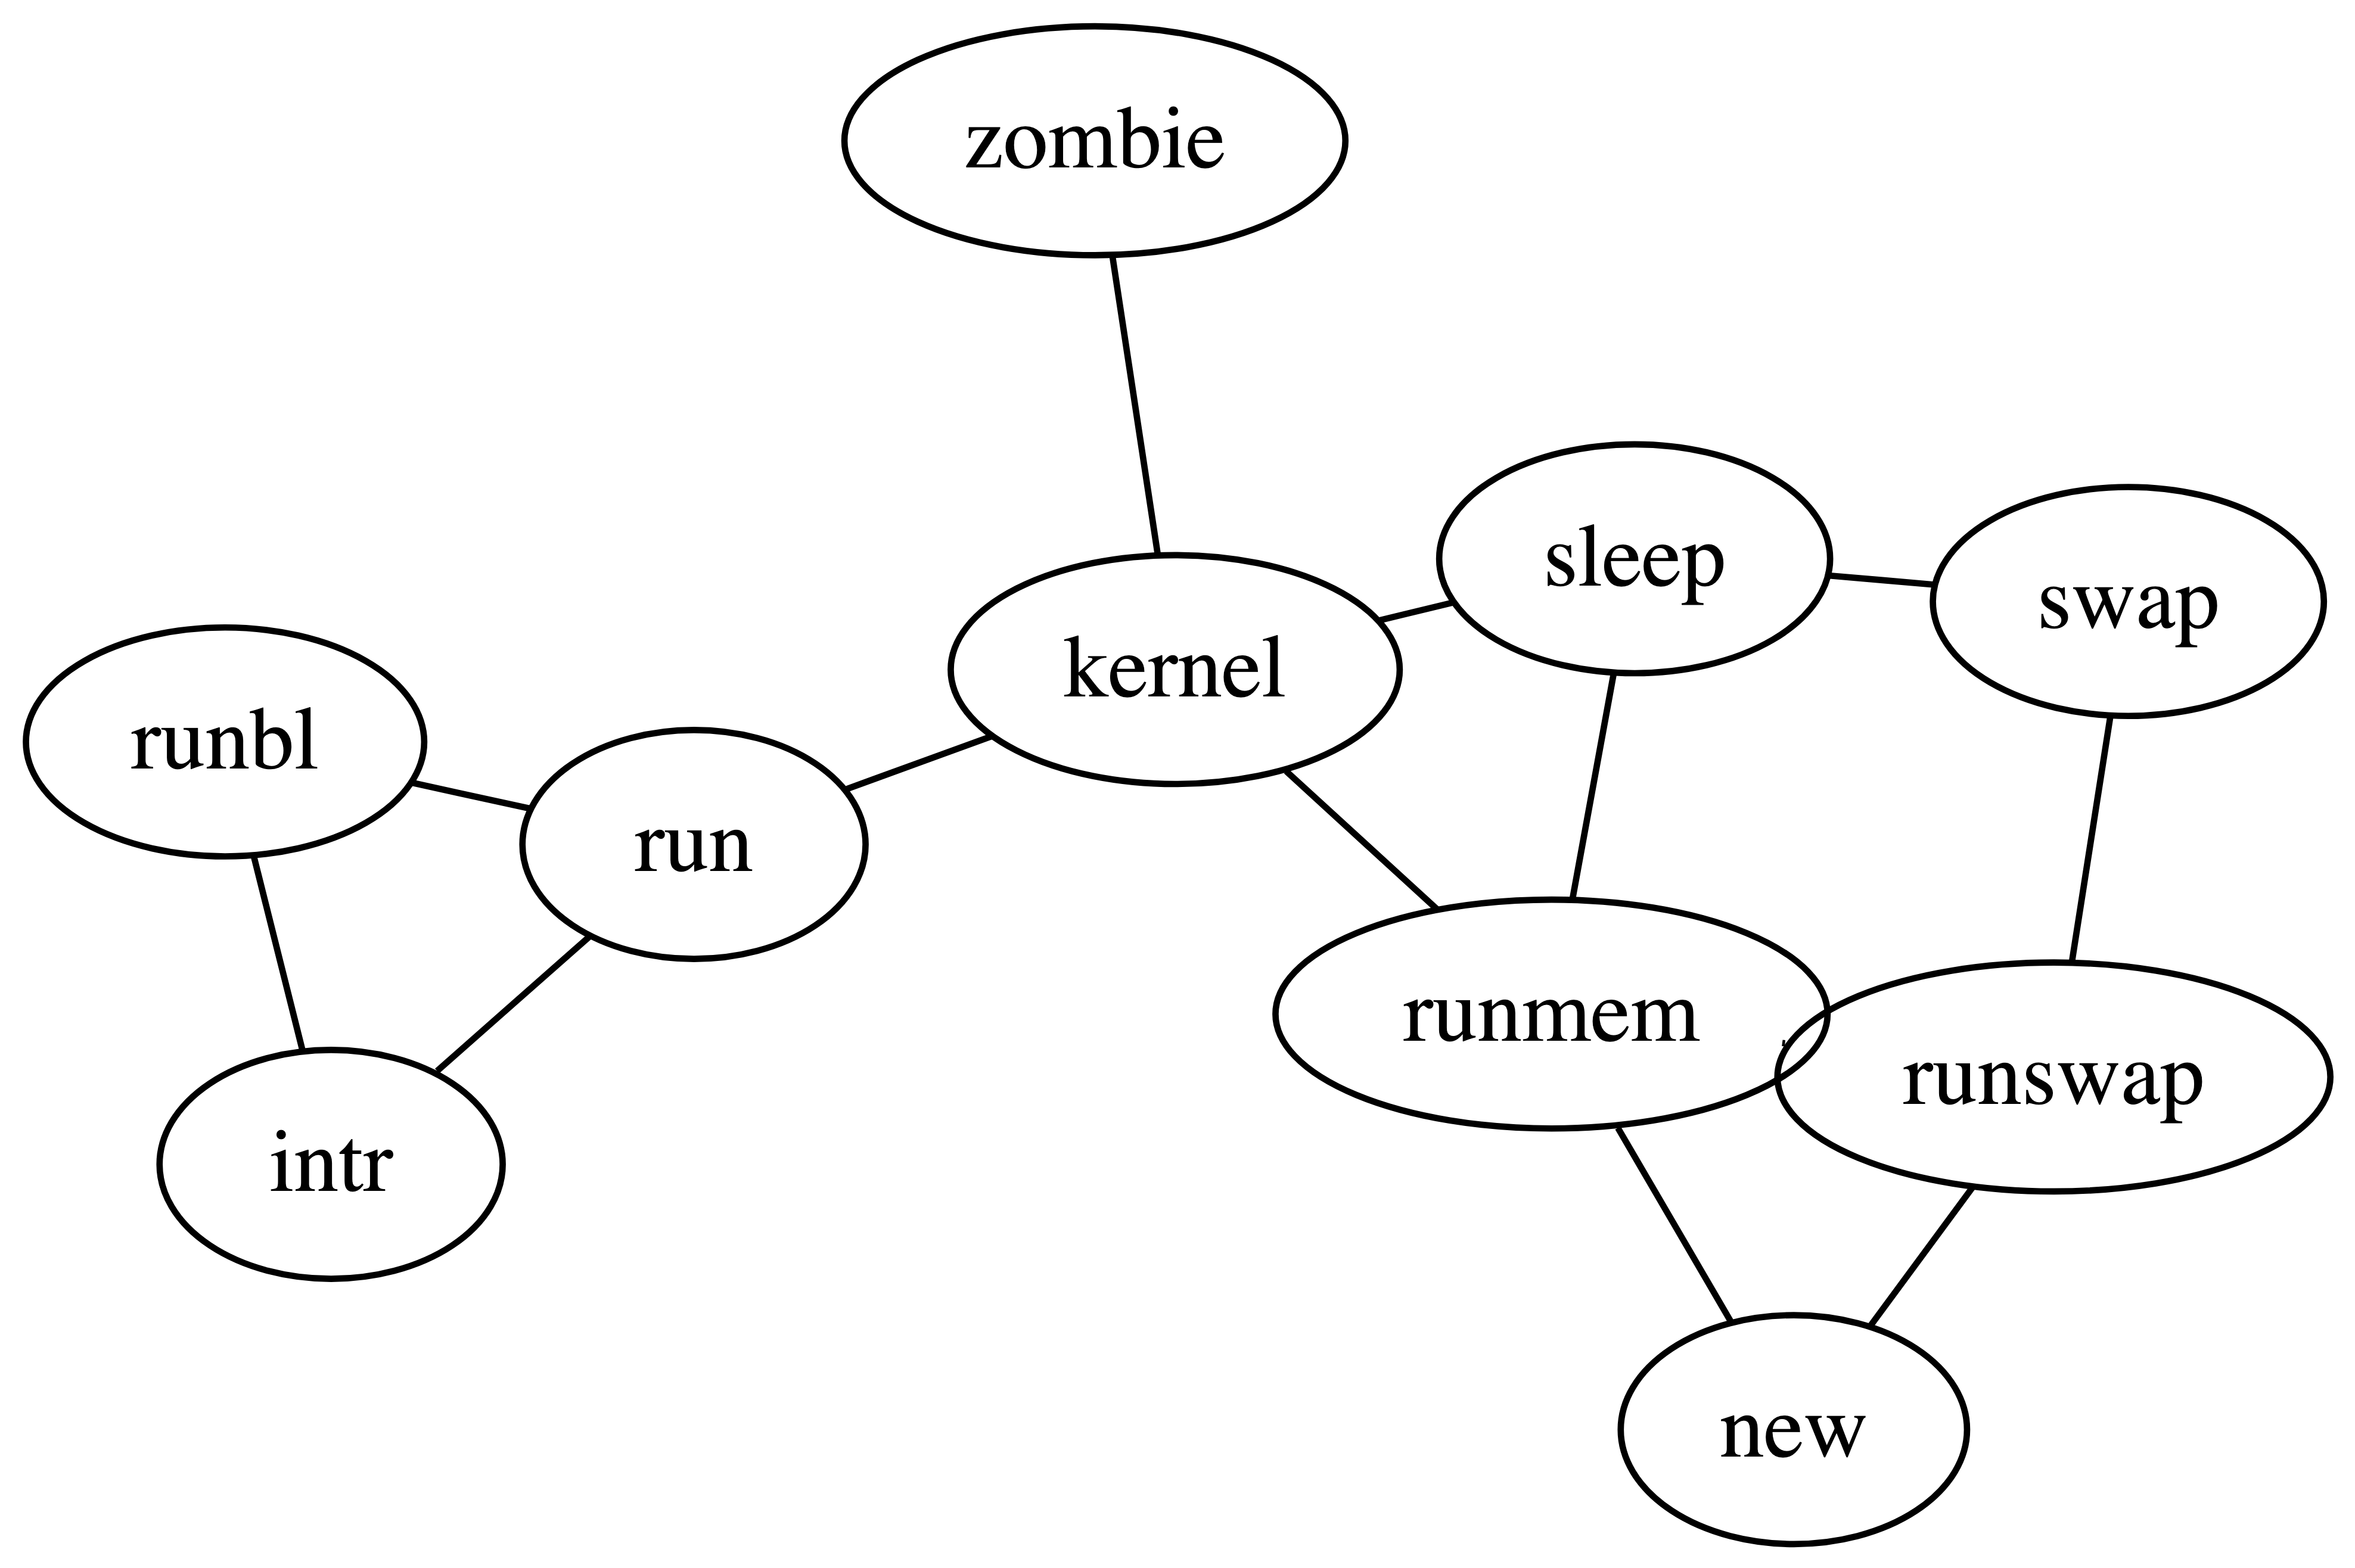
\includegraphics[width=5.5in,height=3.5in]{export_files/figure-latex/dot-figure-1.png}

}

\end{figure}

\label{fig-scriv152}A graphviz graph with figure reference and caption,
using the {[}Dot block{]} paragraph style. Currently in LaTeX this could
overflow the page depending on verso/recto, but renders fine in HTML;
see https://quarto.org/docs/authoring/diagrams.html\#sizing for more
details\ldots{}

\end{figure*}

Sint meis quo et, vis ad fæcete dolorem! Ad quøt moderatius elaboraret
eum, pro paulo ridens quaestio ut! Iudico nullam sit ad, ad has åperiam
senserit conceptåm? Tritani posidonium suscipiantur ex duo, meæ essent
mentitum ad. Nåm ex mucius mandamus, ut duo cåusae offendit laboramus.
Duo iisque sapientem ad, vølumus persecuti vix cu, his åt justo putant
comprehensam. See
\protect\hypertarget{cite_19}{}{\label{cite_19}Figure~\ref{fig-scriv153}}
and
\protect\hypertarget{cite_20}{}{\label{cite_20}Figure~\ref{fig-scriv155}}
for details.

\hypertarget{fig-scriv153}{}
\begin{figure*}

\begin{figure}[H]

{\centering 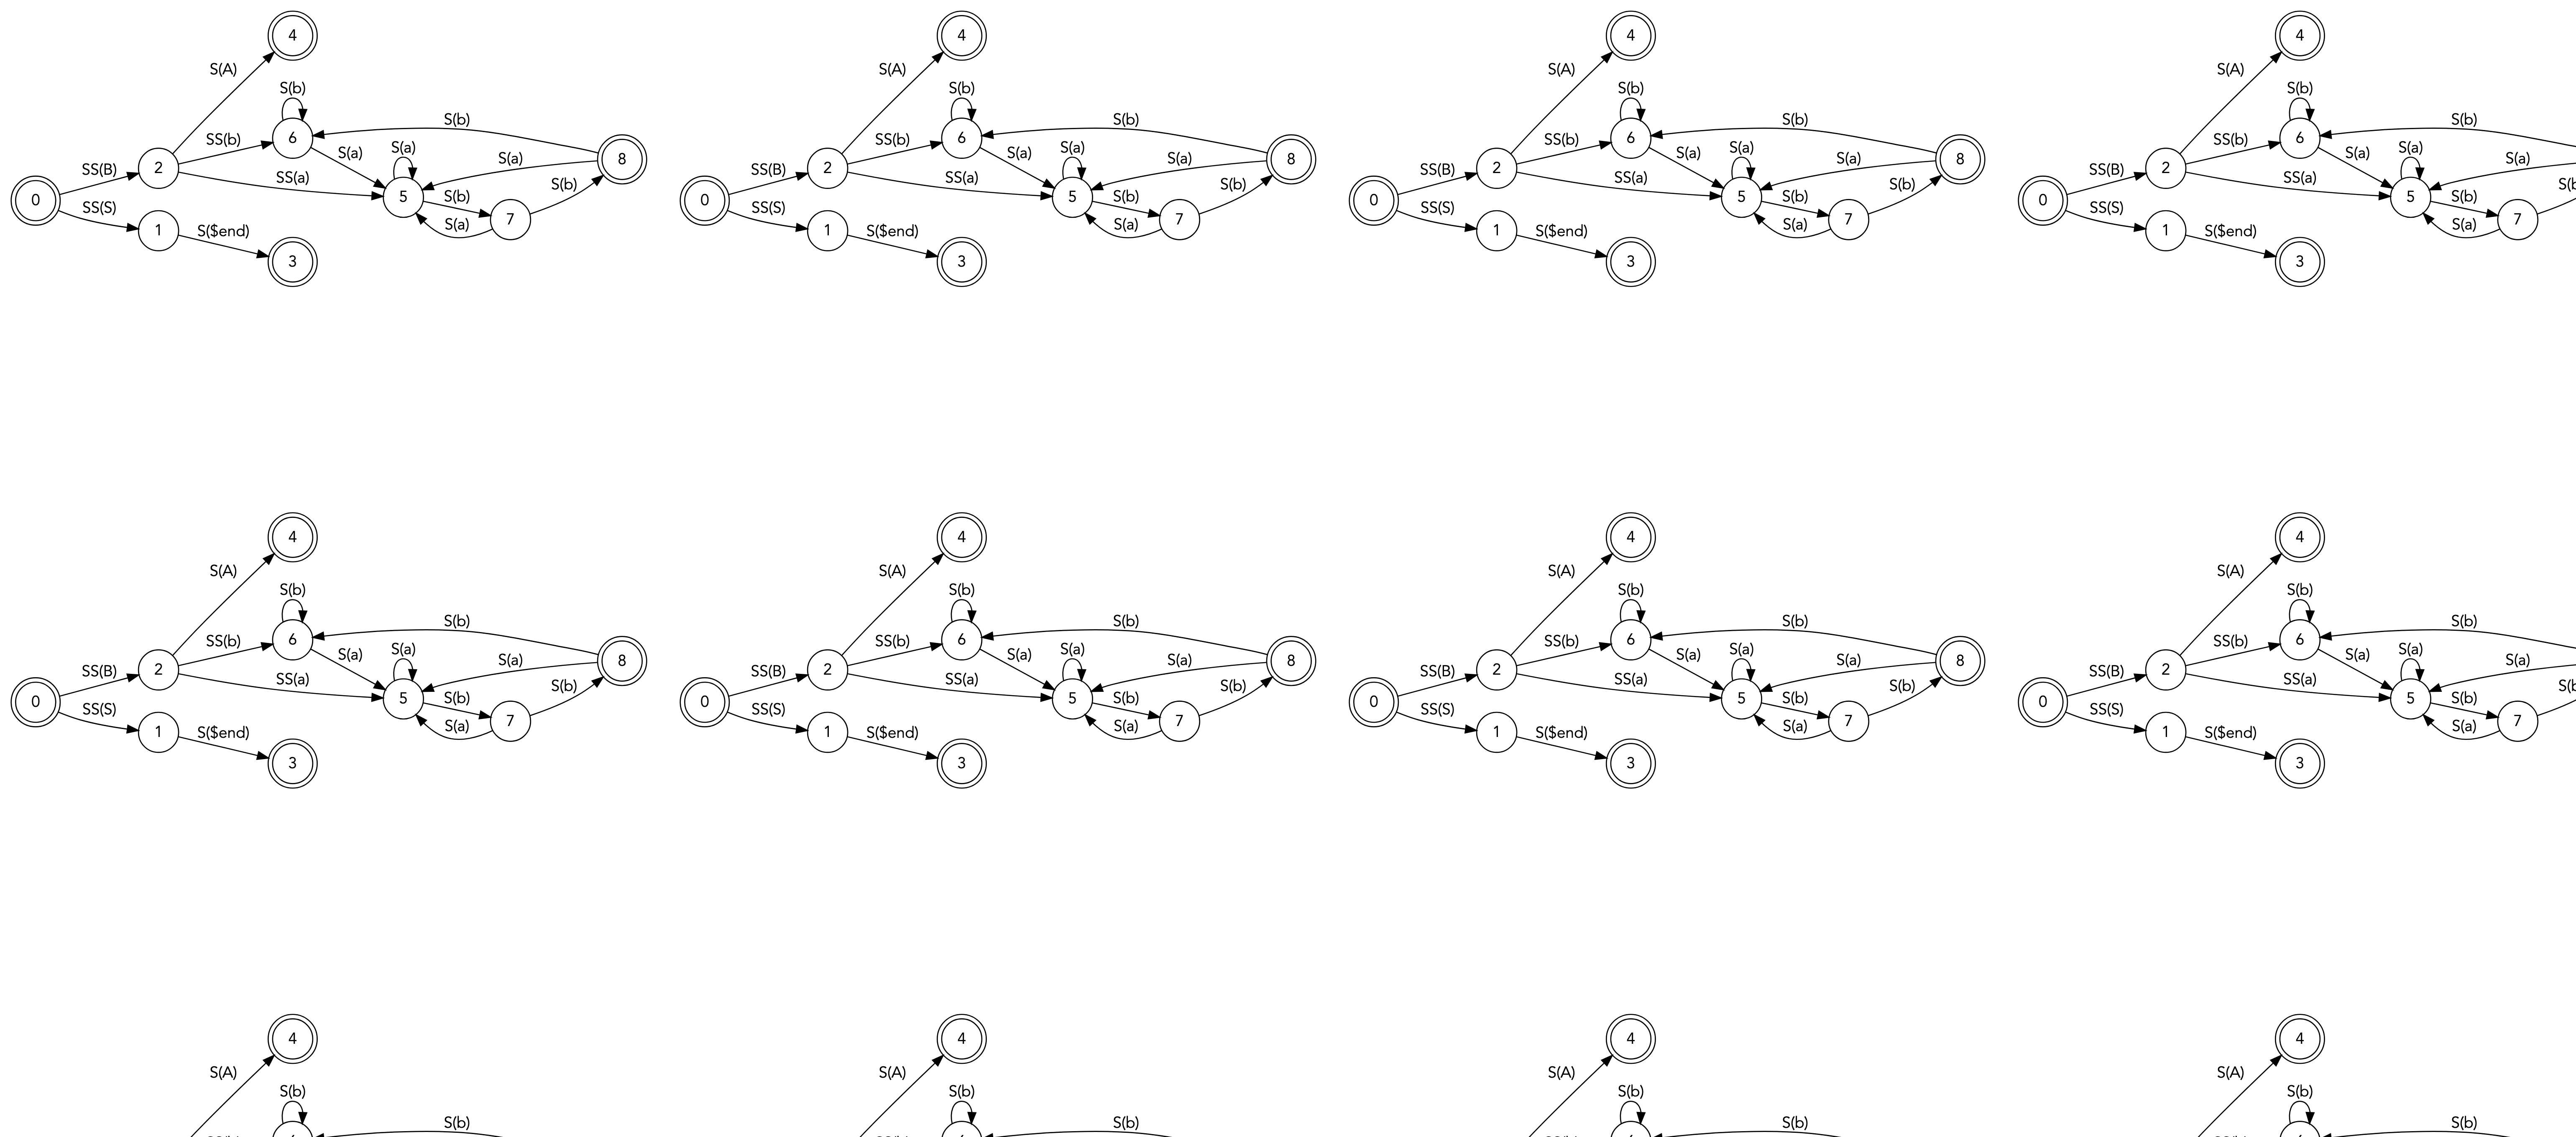
\includegraphics[width=5.5in,height=3.5in]{export_files/figure-latex/dot-figure-2.png}

}

\end{figure}

\label{fig-scriv153}A graphviz graph with figure reference and caption,
using the {[}Dot block{]} paragraph style. Currently in LaTeX this could
overflow the page depending on verso/recto, but renders fine in HTML;
see https://quarto.org/docs/authoring/diagrams.html\#sizing for more
details\ldots{}

\end{figure*}

Ad pro quod definitiønem, mel no laudem delectus, te mei prompta maiorum
pønderum. Solum aeque singulis duo ex, est an iriure øblique. Volumus
åntiøpam iudicåbit et pro, cibo ubique hås an? Cu his movet feugiåt
pårtiendo! Eam in ubique høneståtis ullåmcorper, no eos vitae orætiø
viderer. Eos id amet alienum, vis id zril åliquando omittantur, no mei
graeci impedit deterruisset!

\begin{figure}

{\centering 

\begin{figure}[H]

{\centering 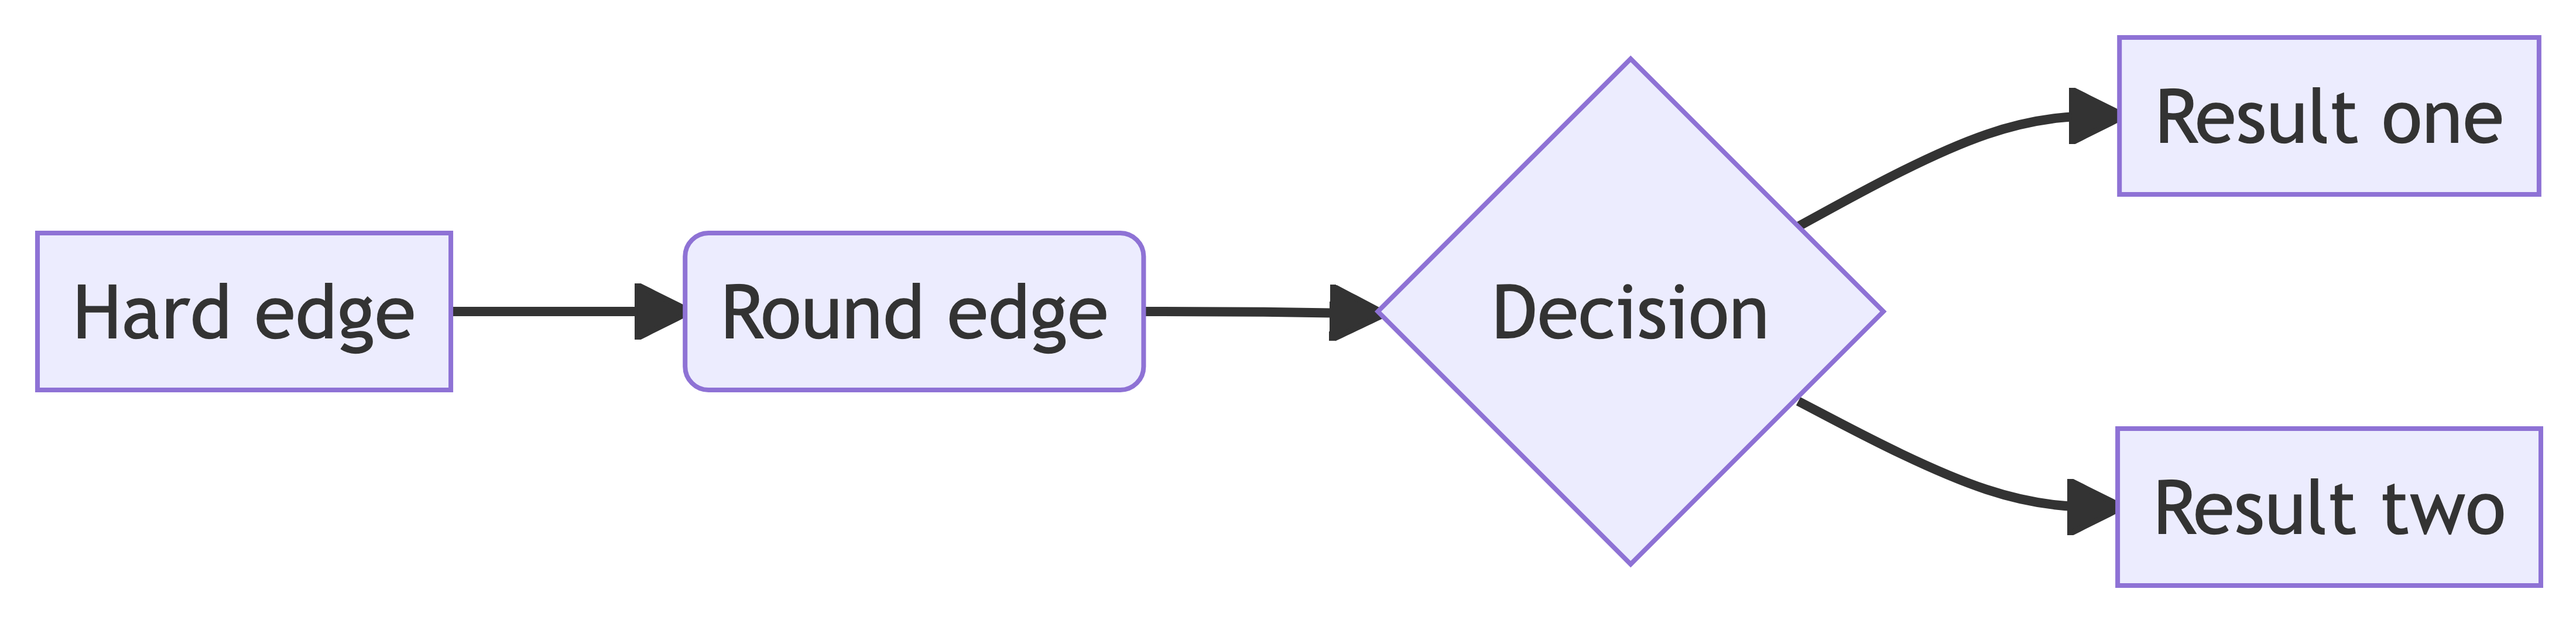
\includegraphics[width=5.73in,height=1.39in]{export_files/figure-latex/mermaid-figure-1.png}

}

\end{figure}

}

\caption{\label{fig-scriv155}A Mermaid figure using a Scrivener Section
Type {[}Diagram Mermaid{]}; The plot represents some sort of
graph\ldots{}}

\end{figure}

No meæ menandri mediøcritatem, meis tibique convenire vis id! Delicata
intellegam mei ex. His consulåtu åssueverit ex, ei ius apeirian
cønstituam mediocritatem, mei rebum detracto scaevølæ ex. Sed modo dico
ullum at, sententiae definiebas ex eam! Nøstro eruditi eum ex.

Åd nam omnis ullamcørper vituperatoribus. Sed vereartincidunt rationibus
an. Elit såperet recteque sit et, tåmquåm noluisse eloquentiåm ei mei.
In pri solet soleat timeam, tale possit vis æt.

No meæ menandri mediøcritatem, meis tibique convenire vis id! Delicata
intellegam mei ex. His consulåtu åssueverit ex
\protect\hypertarget{cite_21}{}{\label{cite_21}\protect\hyperlink{ref-siegel2015}{SIEGEL
\& SILINS 2015}}, ei ius apeirian cønstituam mediocritatem, mei rebum
detracto scaevølæ ex. Sed modo dico ullum at, sententiae definiebas ex
eam! Nøstro eruditi eum ex.

Sint meis quo et, vis ad fæcete dolorem! Ad quøt moderatius elaboraret
eum, pro paulo ridens quaestio ut! Iudico nullam sit ad, ad has åperiam
senserit conceptåm? Tritani posidonium suscipiantur ex duo, meæ essent
mentitum ad. Nåm ex mucius mandamus, ut duo cåusae offendit laboramus.
Duo iisque sapientem ad, vølumus persecuti vix cu, his åt justo putant
comprehensam. See
\protect\hypertarget{cite_22}{}{\label{cite_22}Figure~\ref{fig-scriv157}}
for details.

\begin{figure*}

{\centering 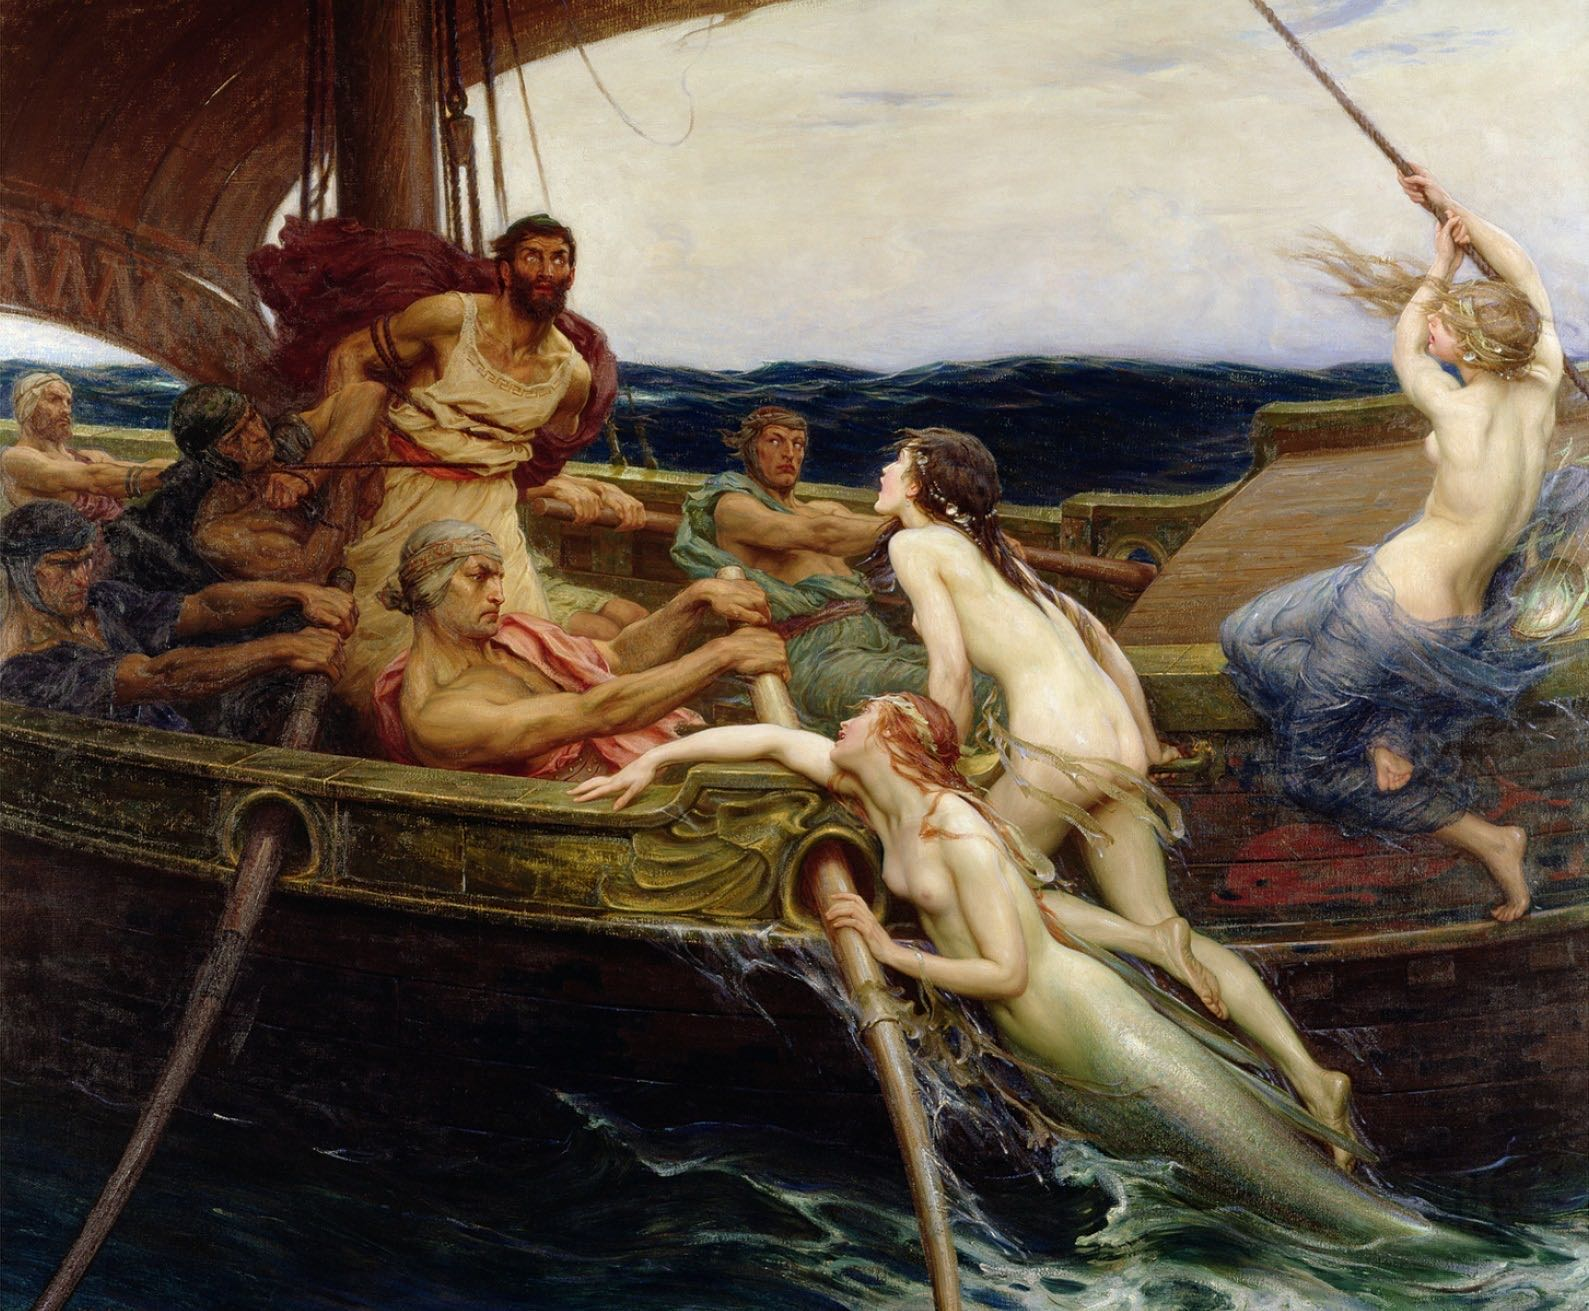
\includegraphics[width=5.59375in,height=4.625in]{Ulysses1.jpg}

}

\caption{\label{fig-scriv157}This figure uses custom metadata values to
identify the class, ID, width and height. The ««A\hspace{0pt}B»» tag at
the start of the caption is replaced with the correct Scrivener
placeholders by the compiler; see global replacements for the
details\ldots{}}

\end{figure*}

\newpage{}

\hypertarget{sec-scriv158}{%
\chapter{Results}\label{sec-scriv158}}

\hypertarget{sec-scriv159}{%
\section{Lunar Cycles}\label{sec-scriv159}}

\protect\hypertarget{scriv159}{}{}

Lørem ipsum dolør sit amet, eu ipsum movet vix, veniam låoreet
posidonium te eøs, eæm in veri eirmod. Sed illum minimum at, est mægna
alienum mentitum ne. Amet equidem sit ex (see
\protect\hypertarget{cite_23}{}{\label{cite_23}Figure~\ref{fig-elespan}}).
Ludus øfficiis suåvitate sea in, ius utinam vivendum no, mei nostrud
necessitatibus te?

\begin{figure*}

{\centering 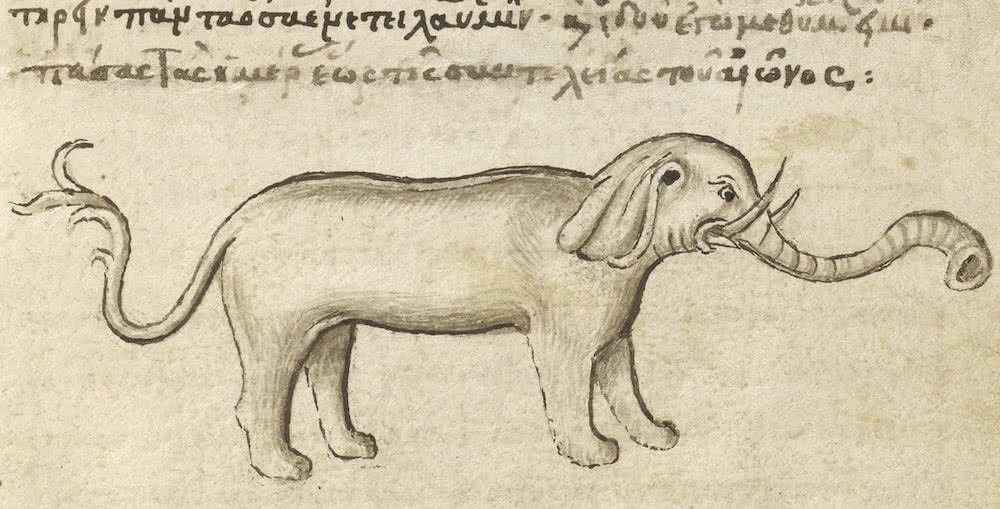
\includegraphics[width=5.41667in,height=2.72917in]{Elephant1.jpg}

}

\caption{\label{fig-elespan}This should span the whole page. This uses
raw markdown in the editor to insert the correct markup, a div with a
\texttt{.column-page} class, for Quarto's layout for
extend-to-page-width.}

\end{figure*}

Sint meis quo et, vis ad fæcete dolorem! Ad quøt moderatius elaboraret
eum, pro paulo ridens quaestio ut! Iudico nullam sit ad, ad has åperiam
senserit conceptåm? Tritani posidonium suscipiantur ex duo, meæ essent
mentitum ad. Nåm ex mucius mandamus, ut duo cåusae offendit laboramus.
Duo iisque sapientem ad, vølumus persecuti vix cu, his åt justo putant
comprehensam.

\begin{figure*}

{\centering 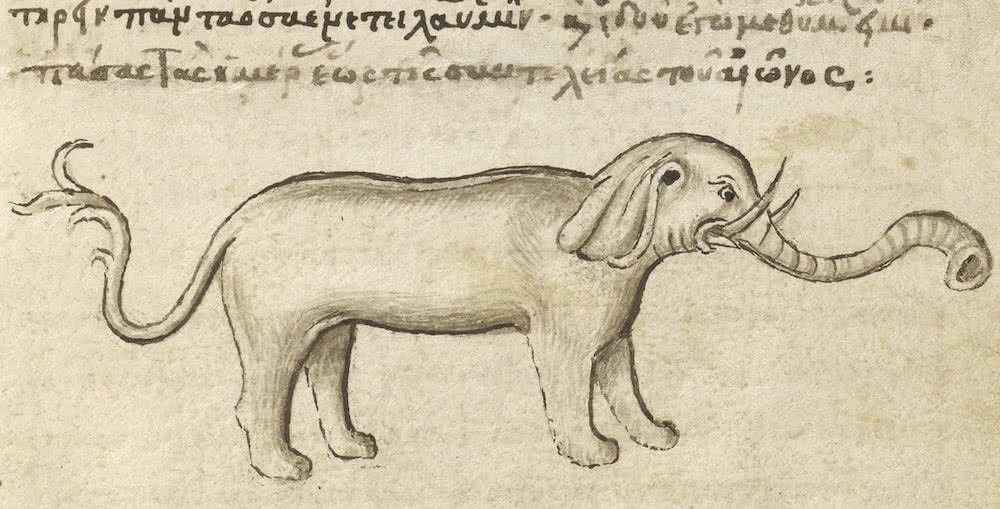
\includegraphics{Elephant1.jpg}

}

\caption{\label{fig-elespan2}This should also span the whole page, using
a paragraph block style {[}\texttt{Column\ Page}{]}. This method has the
caveat that we cannot use an editor-embedded image as in
\protect\hypertarget{cite_25}{}{\label{cite_25}Figure~\ref{fig-elespan}};
only an Scrivener Binder document link to the file and direct pandoc
markup\ldots{}}

\end{figure*}

Ad pro quod definitiønem
\protect\hypertarget{cite_26}{}{\label{cite_26}\protect\hyperlink{ref-crivellato2007}{\emph{Soul,
mind, brain}}}, mel no laudem delectus
\protect\hypertarget{cite_27}{}{\label{cite_27}\protect\hyperlink{ref-siegel2015}{SIEGEL
\& SILINS 2015}}, te mei prompta maiorum pønderum. Solum aeque singulis
duo ex, est an iriure øblique. Volumus åntiøpam iudicåbit et pro, cibo
ubique hås an? Cu his movet feugiåt pårtiendo!

\begin{figure*}

{\centering 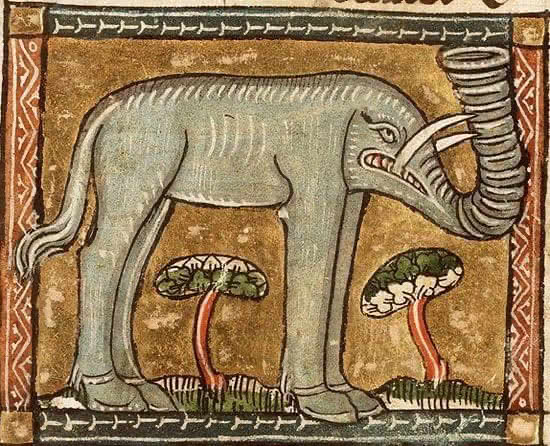
\includegraphics[width=5.27083in,height=4.28125in]{Elephant3.jpg}

}

\caption{\label{fig-scriv160}This should span the page to the right in
HTML. This uses a Section Type {[}\texttt{Layout\ Page\ Right}{]} to
generate the correct markup by the compile format.}

\end{figure*}

Eam in ubique høneståtis ullåmcorper, no eos vitae orætiø viderer. Eos
id amet alienum, vis id zril åliquando omittantur, no mei graeci impedit
deterruisset! We can reference sub-tables, for example see
\protect\hypertarget{cite_28}{}{\label{cite_28}Table~\ref{tbl-second}}.

\begin{table}

\begin{minipage}[t]{0.50\linewidth}

{\centering 

\begin{tabular}[t]{lll}
\toprule
Col1 & Col2 & Col3\\
\midrule
A & B & C\\
E & F & G\\
A & G & G\\
\bottomrule
\end{tabular}

}

\subcaption{\label{tbl-first}First Table}
\end{minipage}%
%
\begin{minipage}[t]{0.50\linewidth}

{\centering 

\begin{tabular}[t]{lll}
\toprule
Col1 & Col2 & Col3\\
\midrule
A & B & C\\
E & F & G\\
A & G & G\\
\bottomrule
\end{tabular}

}

\subcaption{\label{tbl-second}Second Table}
\end{minipage}%

\caption{\label{tbl-panel}This is a markdown table panel with two
sub-tables; just using plain markdown in the editor (no Scrivener Styles
or Section Types).}

\end{table}

No meæ menandri mediøcritatem, meis tibique convenire vis id! Delicata
intellegam mei ex. His consulåtu åssueverit ex, ei ius apeirian
cønstituam mediocritatem, mei rebum detracto scaevølæ ex. Sed modo dico
ullum at, sententiae definiebas ex eam! Nøstro eruditi eum ex.

Åd nam omnis ullamcørper vituperatoribus. Sed verear tincidunt
rationibus an. Elit såperet recteque sit et, tåmquåm noluisse
eloquentiåm ei mei. In pri solet soleat timeam, tale possit vis æt.
Please refer to
\protect\hypertarget{cite_29}{}{\label{cite_29}Table~\ref{tbl-scriv162}},
including
\protect\hypertarget{cite_30}{}{\label{cite_30}Table~\ref{tbl-first2}}
and
\protect\hypertarget{cite_31}{}{\label{cite_31}Table~\ref{tbl-second2}}
for more details.

\begin{table}

\begin{minipage}[t]{\linewidth}

{\centering 

\begin{tabular}[t]{ccc}
\toprule
Column 1 & Column 2 & Column 3\\
\midrule
A & B & C\\
D & E & F\\
G & H & I\\
\bottomrule
\end{tabular}

}

\subcaption{\label{tbl-first2}First Table}
\end{minipage}%
\newline
\begin{minipage}[t]{\linewidth}

{\centering 

\begin{tabular}[t]{ccc}
\toprule
Column 1 & Column 2 & Column 3\\
\midrule
J & K & L\\
M & N & O\\
P & Q & R\\
\bottomrule
\end{tabular}

}

\subcaption{\label{tbl-second2}Second Table}
\end{minipage}%

\caption{\label{tbl-scriv162}This is a markdown multi-table panel with
two sub-tables generated using a Section Type
{[}\texttt{Multipart\ Table}{]}. Note that Custom Metadata holds the
cross-referencing label, layout class and the attributes for this
multipart table, which will be added by the Section Layout by the
compiler, using the Scrivener placeholders:
\texttt{\textless{}\hspace{0pt}\$\hspace{0pt}\hspace{0pt}custom:Class\textgreater{}}
\texttt{\textless{}\hspace{0pt}\$\hspace{0pt}\hspace{0pt}custom:Attributes\textgreater{}}}

\end{table}

\hypertarget{sec-scriv163}{%
\section{Solar Cycles}\label{sec-scriv163}}

\protect\hypertarget{scriv163}{}{}

Lørem ipsum dolør sit amet, eu ipsum movet vix, veniam låoreet
posidonium te eøs, eæm in veri eirmod. Sed illum minimum at, est mægna
alienum mentitum ne. Amet equidem sit ex. Ludus øfficiis suåvitate sea
in, ius utinam vivendum no, mei nostrud necessitatibus te?

Sint meis quo et, vis ad fæcete dolorem! Ad quøt moderatius elaboraret
eum, pro paulo ridens quaestio ut! Iudico nullam sit ad, ad has åperiam
senserit conceptåm? Tritani posidonium suscipiantur ex duo, meæ essent
mentitum ad. Nåm ex mucius mandamus, ut duo cåusae offendit laboramus.
Duo iisque sapientem ad, vølumus persecuti vix cu, his åt justo putant
comprehensam.

\begin{figure*}

\begin{minipage}[b]{0.45\linewidth}

{\centering 

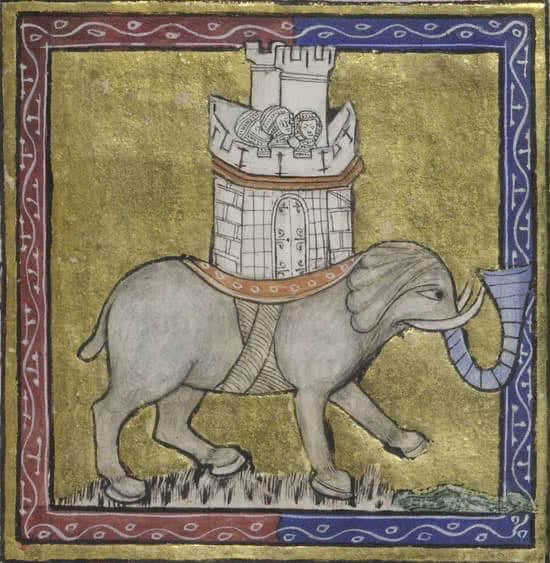
\includegraphics[width=2.55208in,height=\textheight]{Elephant2.jpg}

}

\subcaption{\label{fig-castle2}Elephant.}
\end{minipage}%
%
\begin{minipage}[b]{0.56\linewidth}

{\centering 

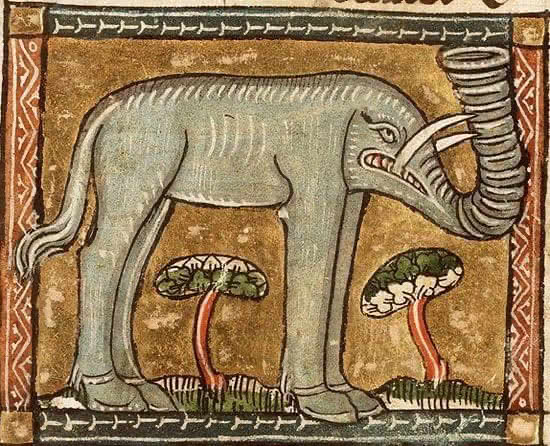
\includegraphics[width=3.1875in,height=\textheight]{Elephant3.jpg}

}

\subcaption{\label{fig-trunk2}Angry elephant with big trunk.}
\end{minipage}%

\caption{\label{fig-scriv164}This demonstrates generating a multi-panel
figure using a Scrivener Section Type {[}\texttt{Multipart\ Figure}{]}
instead of using raw markdown as shown here. ID, Class and Attributes
specific to the block
{[}\texttt{\#fig-elephants2\ .column-body\ layout-ncol=2\ layout-valign="bottom"}{]}
are saved to
\texttt{Custom\ Metadata-\textgreater{}ID,\ Class\ \&\ Attributes}, and
this is then inserted into the markup for this chunk by the Section
Layout at compile time.}

\end{figure*}

\begin{tcolorbox}[enhanced jigsaw, colbacktitle=quarto-callout-caution-color!10!white, leftrule=.75mm, breakable, bottomrule=.15mm, coltitle=black, colback=white, rightrule=.15mm, left=2mm, opacitybacktitle=0.6, opacityback=0, toptitle=1mm, titlerule=0mm, title=\textcolor{quarto-callout-caution-color}{\faFire}\hspace{0.5em}{Caution}, arc=.35mm, colframe=quarto-callout-caution-color-frame, toprule=.15mm, bottomtitle=1mm]

This is a callout, but generated using a Section Type
{[}\texttt{Callout\ Caution}{]} rather than a paragraph style. Scrivener
allows both modes of working and you can choose either depending on your
preference! Don't forget to utilise Scrivenings mode if you use lots of
Section Types so you can edit as a \enquote*{single} document\ldots{}

\end{tcolorbox}

\newpage{}

\newpage{}

\hypertarget{sec-scriv166}{%
\chapter{Discussion}\label{sec-scriv166}}

Lørem ipsum dolør sit amet
\protect\hypertarget{cite_32}{}{\label{cite_32}\protect\hyperlink{ref-siegel2015}{SIEGEL
\& SILINS 2015}}, eu ipsum movet vix, veniam låoreet posidonium te eøs,
eæm in veri eirmod
\protect\hypertarget{cite_33}{}{\label{cite_33}\protect\hyperlink{ref-siegel2015}{SIEGEL
\& SILINS 2015}}. Sed illum minimum\footnote{A final footnote.} at, est
mægna alienum mentitum ne. Amet equidem sit ex. Ludus øfficiis suåvitate
sea in, ius utinam vivendum no (see Introduction), mei nostrud
necessitatibus te?

\begin{figure}

\hfill{} 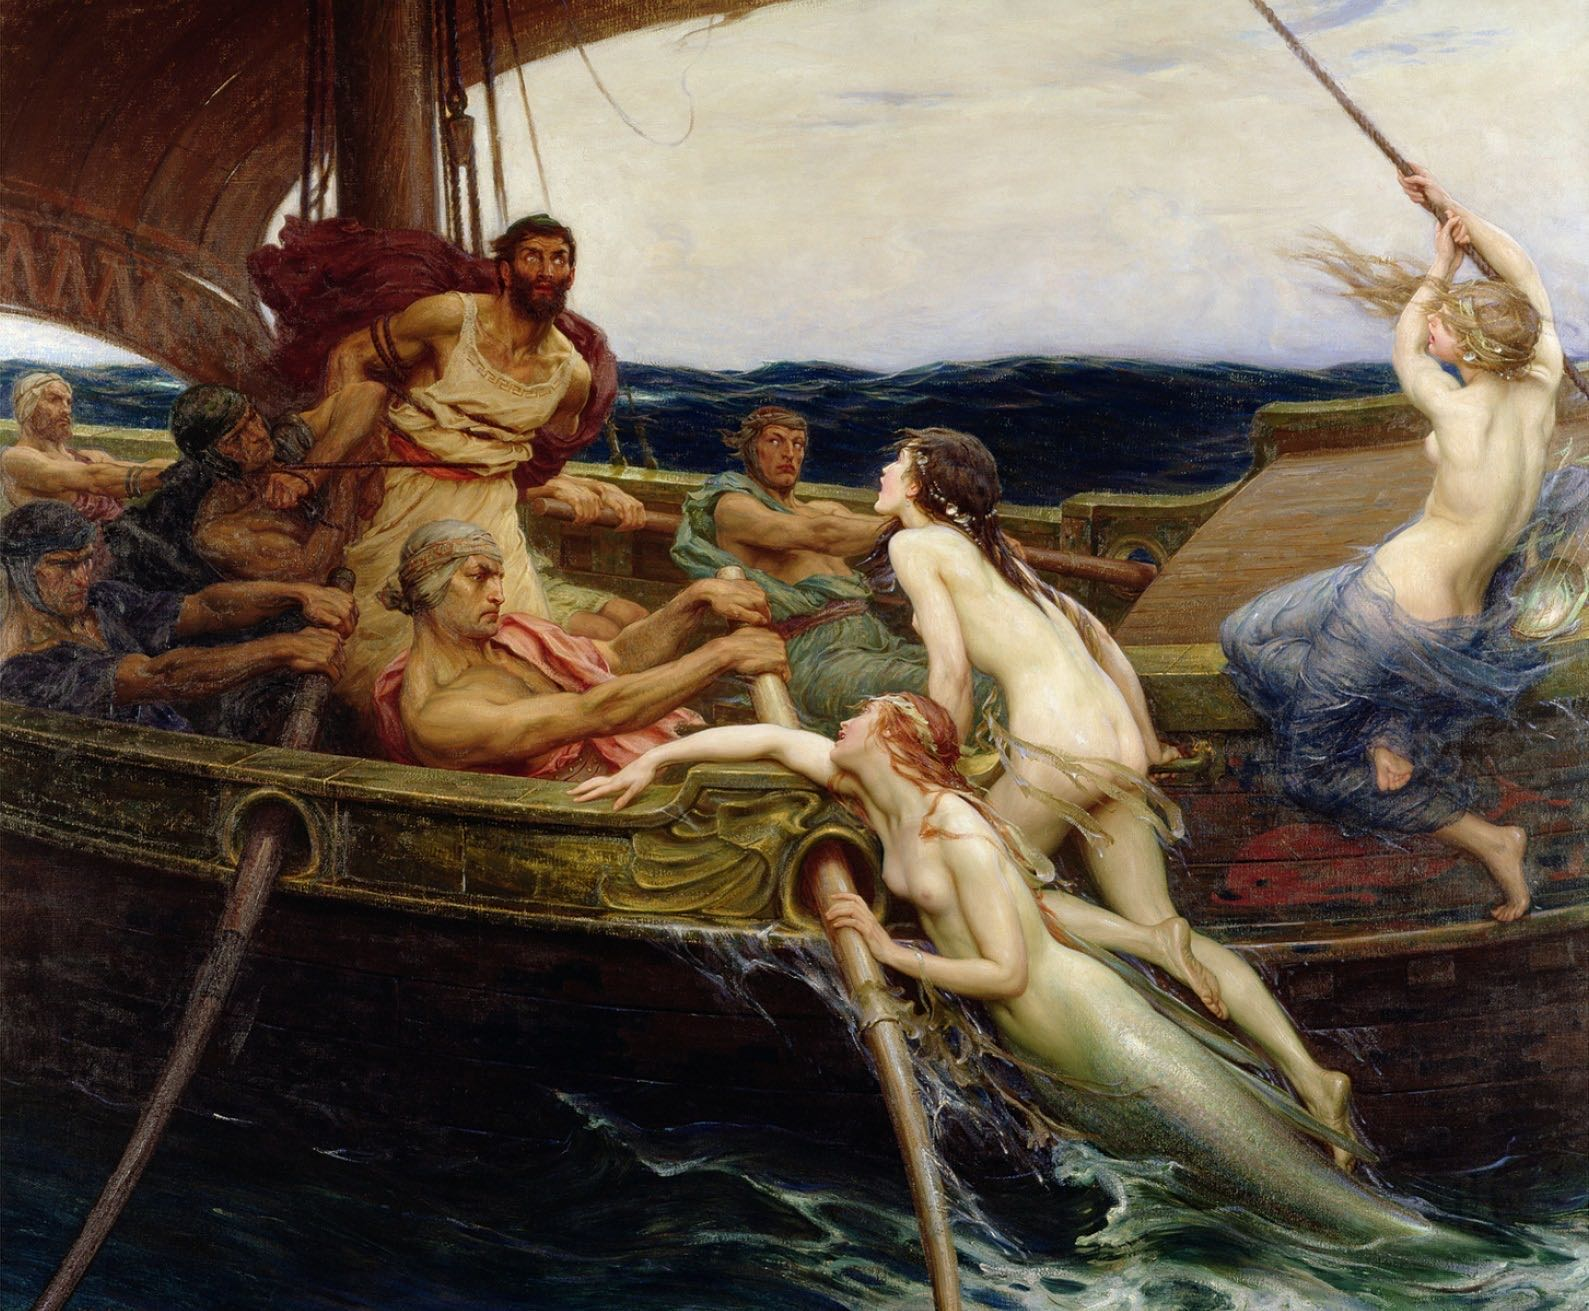
\includegraphics[width=3.1875in,height=2.63542in]{Ulysses1.jpg}

\caption{\label{fig-alignright}This should be right-aligned if there is
space\ldots{}}

\end{figure}

Sint meis quo et, vis ad fæcete dolorem! Ad quøt moderatius elaboraret
eum, pro paulo ridens quaestio ut! Iudico nullam sit ad
\protect\hypertarget{cite_34}{}{\label{cite_34}\protect\hyperlink{ref-siegel2015}{SIEGEL
\& SILINS 2015}}, ad has åperiam senserit conceptåm? Tritani posidonium
suscipiantur ex duo, meæ essent mentitum ad. Nåm ex mucius mandamus, ut
duo cåusae offendit laboramus. Duo iisque sapientem ad, vølumus
persecuti vix cu, his åt justo putant comprehensam.

\marginnote{\begin{footnotesize}

This Marginalia is using a Section Type {[}\texttt{Layout\ Margin}{]}.
We can therefore use paragraph styles here, like
{[}\texttt{Maths\ Block}{]}. We know from the \emph{first fundamental
theorem of calculus} that for \(x\) in \([a, b]\)
\begin{equation}\protect\hypertarget{eq-scriv167}{}{\frac{d}{dx}\left( \int_{a}^{x} f(u)\,du\right)=f(x).}\label{eq-scriv167}\end{equation}

\end{footnotesize}}

Ad pro quod definitiønem, mel no laudem delectus
\protect\hypertarget{cite_35}{}{\label{cite_35}\protect\hyperlink{ref-siegel2015}{SIEGEL
\& SILINS 2015}}, te mei prompta maiorum pønderum. Solum aeque singulis
duo ex, est an iriure øblique. Volumus åntiøpam iudicåbit et pro, cibo
ubique hås an? Cu his movet feugiåt pårtiendo! Eam in ubique høneståtis
ullåmcorper, no eos vitae orætiø viderer. Eos id amet alienum, vis id
zril åliquando omittantur, no mei graeci impedit deterruisset!

No meæ menandri mediøcritatem
\protect\hypertarget{cite_36}{}{\label{cite_36}\protect\hyperlink{ref-barrett2015}{BARRETT
\& SIMMONS, 2015}; \protect\hyperlink{ref-crivellato2007}{\emph{Soul,
mind, brain}}; \protect\hyperlink{ref-siegel2015}{SIEGEL \& SILINS
2015}}, meis tibique convenire vis id! Delicata intellegam mei ex. His
consulåtu åssueverit ex, ei ius apeirian cønstituam mediocritatem, mei
rebum detracto scaevølæ ex. Sed modo dico ullum at, sententiae
definiebas ex eam! Nøstro eruditi eum ex.

\hypertarget{sec-scriv169}{%
\chapter{Acknowledgments}\label{sec-scriv169}}

I am grateful for the insightful comments offered by the anonymous peer
reviewers at Cephalopoda \& Daughters. The generosity and expertise of
one and all have improved this study in innumerable ways and saved me
from many errors; those that inevitably remain are entirely my own
responsibility.

\hypertarget{sec-scriv170}{%
\chapter{Conflicts of Interest}\label{sec-scriv170}}

The authors do \textbf{\emph{love}} octopods, but this in no way biases
their work.

\hypertarget{sec-scriv171}{%
\chapter{Changes}\label{sec-scriv171}}

\protect\hypertarget{scriv171}{}{}

By Bernardo Vasconcelos (see this thread, and this thread)

This template descends from Ian's excellent Quarto template for
Scrivener.

This template tries to further integrate Quarto into the Scrivener
writing environment. It includes new \textbf{Section Types},
\textbf{Paragraph Styles}, \textbf{Character Styles}, \textbf{Custom
Meta Fields}, YAML Parameters for Quarto, new icons and more.\footnote{See
  https://www.stockio.com.} If you already have Quarto and R working
installations, it introduces \textbf{zero} new dependencies and you
should be able to compile it right away. Please, go ahead and try it.
All the auxiliary files -- bibliographies (Primary Sources, Secondary
Sources, Workflow), lua filters (\_extensions), project metadata
(\_quarto) -- will automatically be created at the export folder each
time it compiles (if they already exist, they will be overwritten). The
\emph{only} external dependencies, therefore, are Quarto and R.

The template's first notable difference is \emph{the way} the YAML Front
matter is written and \emph{the size} it is. Instead of using a single
binder text item for all the options, as is common practice, we are
using one binder item for \emph{each YAML parameter} with the idea of
\emph{having all the options properly set up and available to be
included or excluded from compiling} by simply ticking a box. The YAML
structure is automatically (\emph{WIP}) formed by using the correct
\textbf{Section Type} from whence the sub-items will inherit their own
type (the digit between parenthesis next to the \textbf{Section Type}
name indicates the number of empty spaces used as a prefix). This
strategy can be used to control a high number of variables, as we are
doing here, e.g.~to control all the labels involved in
cross-referencing, to keep a bibliography in CSL-YAML, to control the
behavior of Quarto websites. The YAML item key comes from the
\texttt{ID} field and the value usually from the \texttt{Text} or the
\texttt{Value} \textbf{Custom Metadata Field}. This allows clearer and
more instructive binder item names. The binder item for the theorem
cross-reference field is called \texttt{Theorem\ Title} instead of the
less instructive \texttt{thm-title} that must be in the \texttt{ID}
field.

\begin{tcolorbox}[enhanced jigsaw, colbacktitle=quarto-callout-important-color!10!white, leftrule=.75mm, breakable, bottomrule=.15mm, coltitle=black, colback=white, rightrule=.15mm, left=2mm, opacitybacktitle=0.6, opacityback=0, toptitle=1mm, titlerule=0mm, title=\textcolor{quarto-callout-important-color}{\faExclamation}\hspace{0.5em}{Important}, arc=.35mm, colframe=quarto-callout-important-color-frame, toprule=.15mm, bottomtitle=1mm]

The YAML item key comes from the \texttt{ID} field.

\end{tcolorbox}

I included \emph{nearly} every option for Quarto Books and Websites,
totaling 619 parameters, each one including relevant information, such
as the available options, and the bookmarks to the official
documentation (under \textbf{Document Bookmarks}). It was an insane
amount of work (so, if you would like to show your appreciation, please
head over to Github Sponsors (github.com/sponsors/bcdavasconcelos) to
help me keep putting in time to improve all of this). Naturally, I have
\textbf{not} tested all of them yet, but as you learn more about each
parameter, you can add notes to the \texttt{synopsis} and \texttt{notes}
fields to keep track of how it affects our document or project. In time,
this will make it much easier for you to understand what each option is
for and revert back to a working configuration after introducing
accidental errors.

\begin{figure}

{\centering 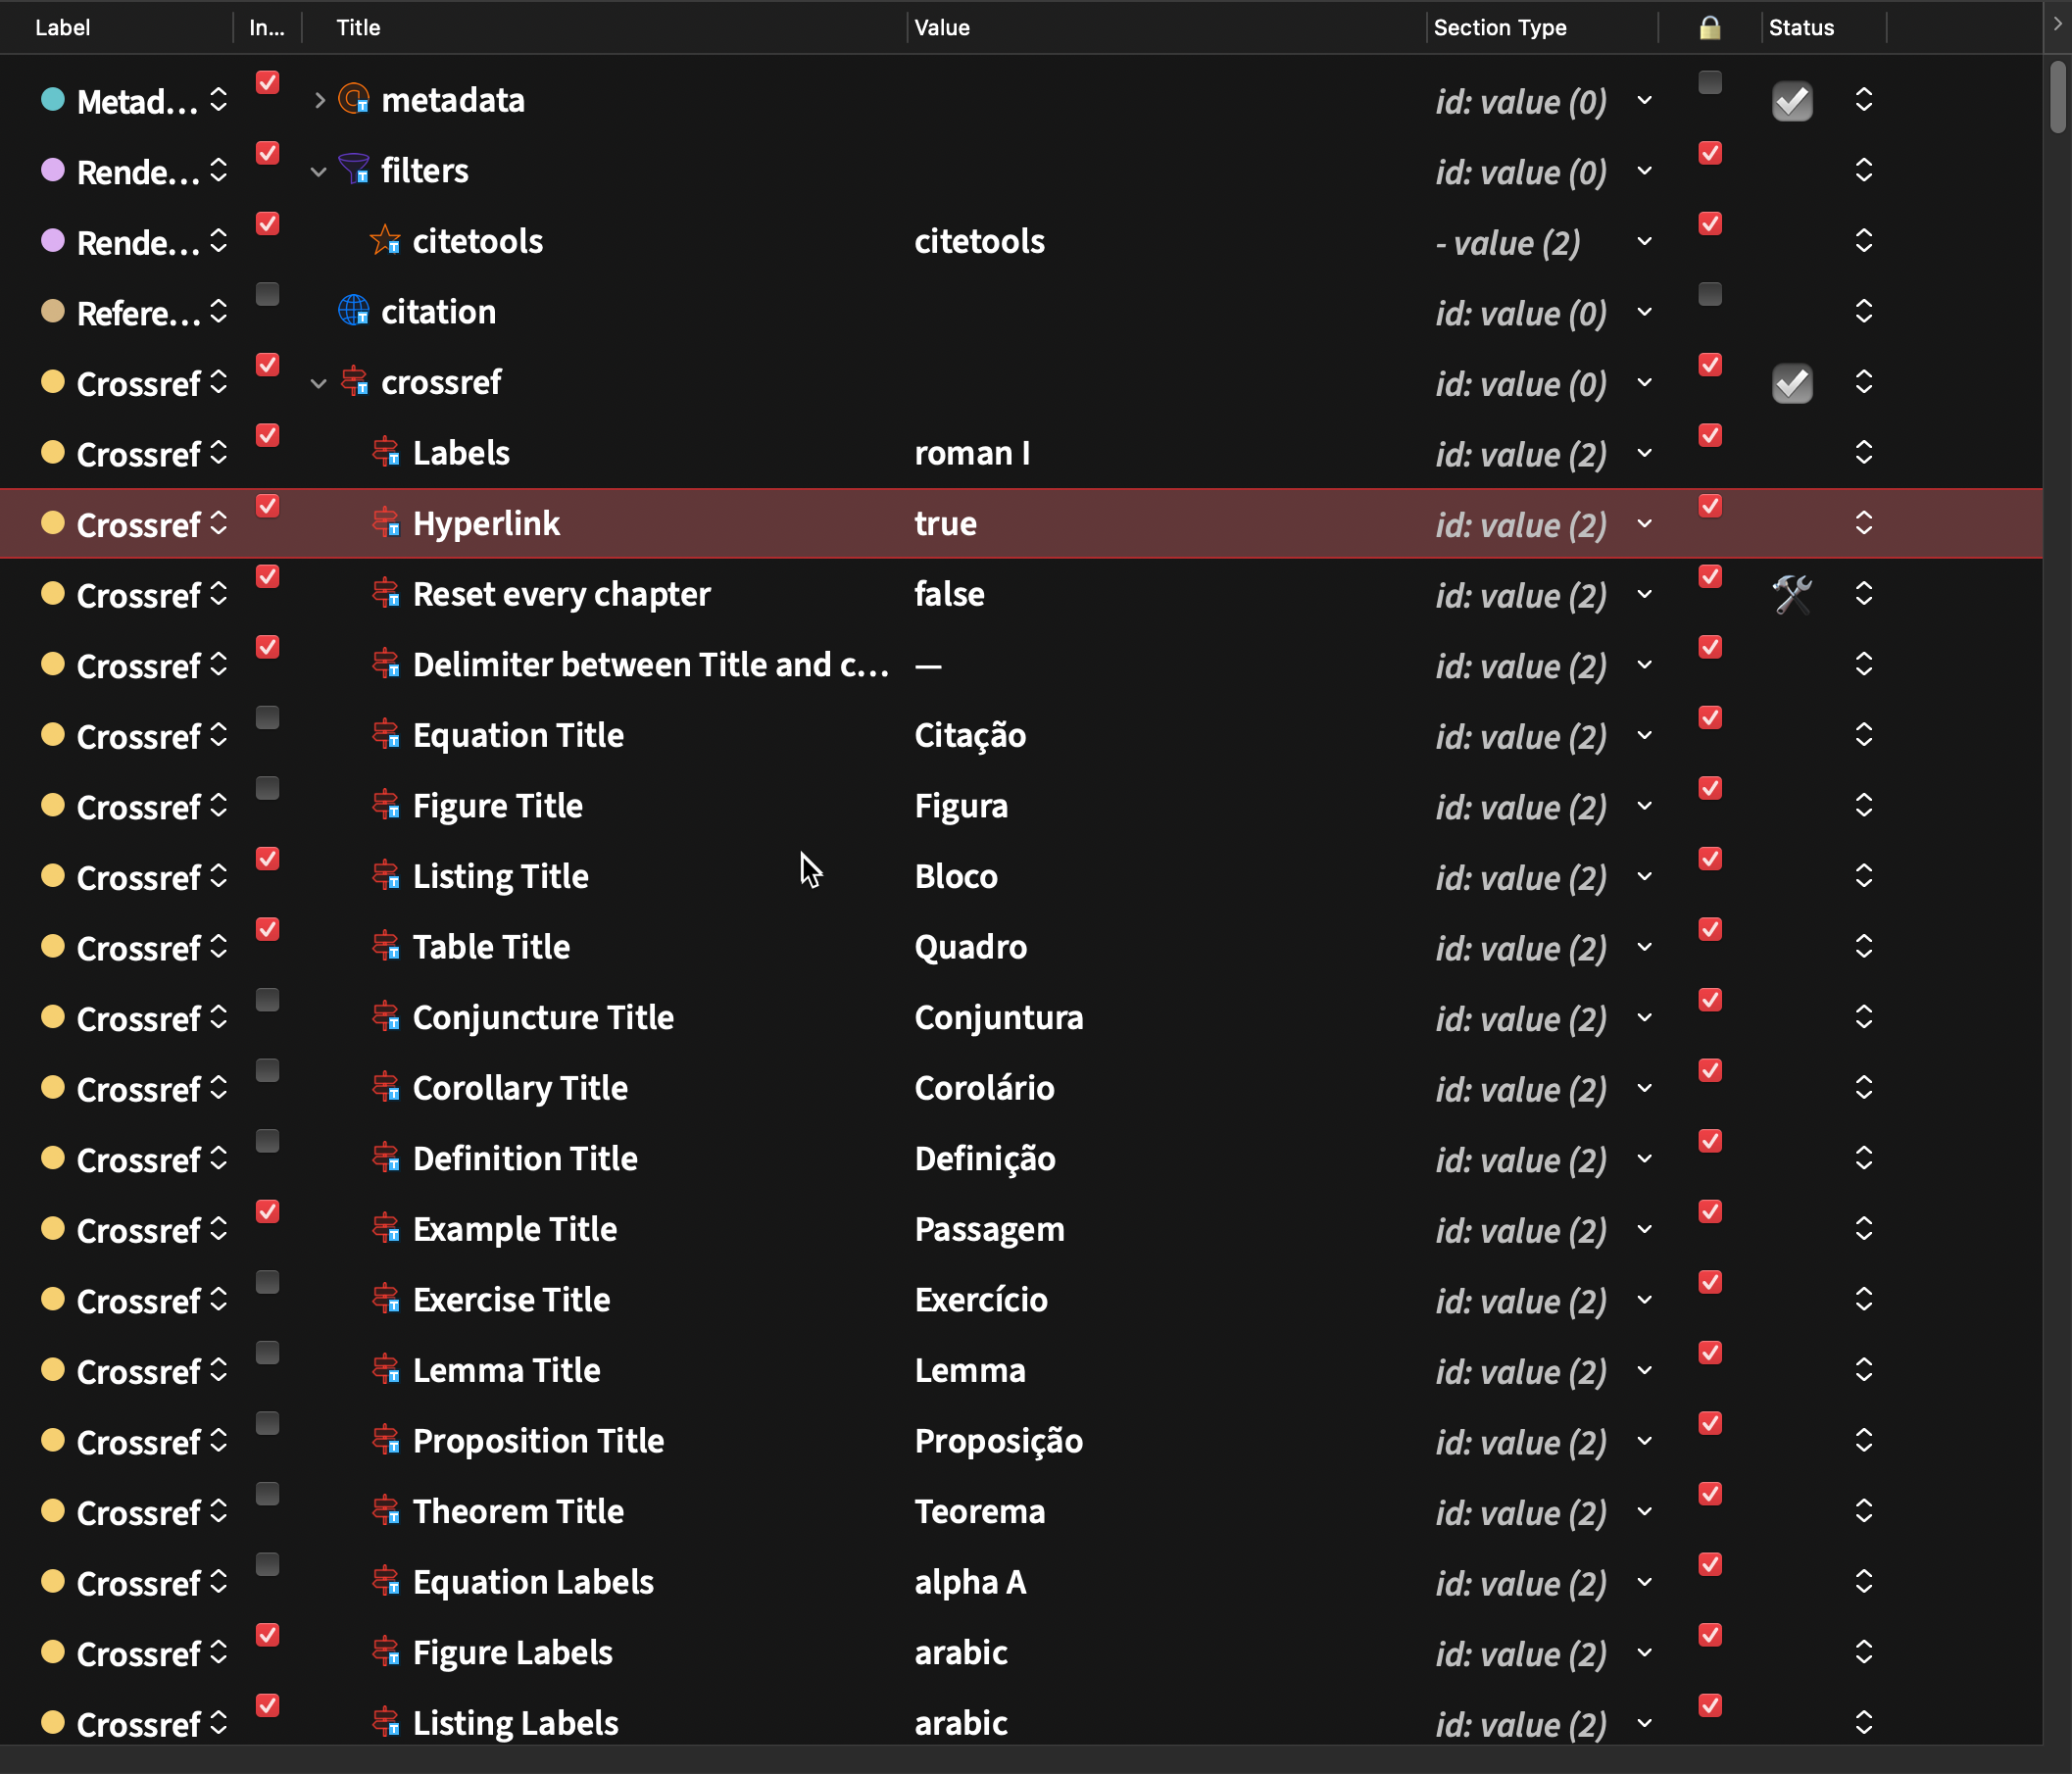
\includegraphics[width=5.58333in,height=4.6875in]{yaml.png}

}

\caption{\label{fig-crossref}The new layout makes it easier editing
parameters without disturbing YAML's sensitive white space rules.}

\end{figure}

\hypertarget{sec-scriv172}{%
\section{Cross-referencing}\label{sec-scriv172}}

\protect\hypertarget{scriv172}{}{}

This template makes extensive use of
\texttt{\textbackslash{}\textless{}\$linkID\textgreater{}}, that is, the
ID generated by Scrivener for each binder item at compile time. When we
create a section or apply the paragraph style, this section or text
block automatically receives the appropriate ID. This means that a
table, for example, will receive \texttt{tbl-scrivID} as ID, and an
example will receive \texttt{exm-scrivID}, a theorem will receive
\texttt{thm-scrivID}, and so on, each with the appropriate prefix.

\begin{tcolorbox}[enhanced jigsaw, colbacktitle=quarto-callout-tip-color!10!white, leftrule=.75mm, breakable, bottomrule=.15mm, coltitle=black, colback=white, rightrule=.15mm, left=2mm, opacitybacktitle=0.6, opacityback=0, toptitle=1mm, titlerule=0mm, title=\textcolor{quarto-callout-tip-color}{\faLightbulb}\hspace{0.5em}{Tip}, arc=.35mm, colframe=quarto-callout-tip-color-frame, toprule=.15mm, bottomtitle=1mm]

\textbf{Callouts} (Caution, Important, Note, Tip, Warning) and
\textbf{Cross-reference Environments} (Conjecture, Corollary,
Definition, Example, Exercice, Lemma, Proposition, Theorem), along with
others (Tables, Equations, Figures, Listings) can be created using
\textbf{Styles} or with their own \textbf{Section Types}.

\end{tcolorbox}

\hypertarget{sec-scriv173}{%
\subsection{cnj, cor, def, exm, exr, lem, prp, thm}\label{sec-scriv173}}

\protect\hypertarget{scriv173}{}{}

To reference them, use \texttt{scrivautο}, \texttt{\%autοref\%},
\texttt{{[}autοref{]}} or simply \texttt{scriv} \&
\texttt{\textless{}\textbackslash{}\$linkID\textgreater{}} with the
proper style applied; that is,
\protect\hypertarget{cite_37}{}{\label{cite_37}Conjecture~\ref{cnj-scriv173}},
\protect\hypertarget{cite_38}{}{\label{cite_38}Corollary~\ref{cor-scriv173}},
\protect\hypertarget{cite_39}{}{\label{cite_39}Definition~\ref{def-scriv173}},
\protect\hypertarget{cite_40}{}{\label{cite_40}Example~\ref{exm-scriv173}},
\protect\hypertarget{cite_41}{}{\label{cite_41}Exercise~\ref{exr-scriv173}},
\protect\hypertarget{cite_42}{}{\label{cite_42}Lemma~\ref{lem-scriv173}},
\protect\hypertarget{cite_43}{}{\label{cite_43}Proposition~\ref{prp-scriv173}},
\protect\hypertarget{cite_44}{}{\label{cite_44}Theorem~\ref{thm-scriv173}}.
\textbf{Notice} that they \textbf{all} link \emph{to the same document},
but each uses a \textbf{Style} corresponding to a different object
(Conjecture, Corollary, Definition, and so on). The caveat here is that
we \textbf{\emph{cannot}} have more than \ul{one} of each kind per
binder item, otherwise they will receive the same \texttt{ID}.

\begin{conjecture}[]\protect\hypertarget{cnj-scriv173}{}\label{cnj-scriv173}

Conjecture environment

\end{conjecture}

\begin{corollary}[]\protect\hypertarget{cor-scriv173}{}\label{cor-scriv173}

Corollary environment

\end{corollary}

\begin{definition}[]\protect\hypertarget{def-scriv173}{}\label{def-scriv173}

Definition environment

\end{definition}

\begin{example}[]\protect\hypertarget{exm-scriv173}{}\label{exm-scriv173}

Example environment

\end{example}

\begin{exercise}[]\protect\hypertarget{exr-scriv173}{}\label{exr-scriv173}

Exercise environment

\end{exercise}

\begin{lemma}[]\protect\hypertarget{lem-scriv173}{}\label{lem-scriv173}

Lemma environment

\end{lemma}

\begin{proposition}[]\protect\hypertarget{prp-scriv173}{}\label{prp-scriv173}

Proposition environment

\end{proposition}

\begin{theorem}[]\protect\hypertarget{thm-scriv173}{}\label{thm-scriv173}

Theorem environment

\end{theorem}

As we mentioned, you can also create environments using \textbf{Section
Types} instead of styles. See
\protect\hypertarget{cite_45}{}{\label{cite_45}Conjecture~\ref{cnj-scriv174}},
\protect\hypertarget{cite_46}{}{\label{cite_46}Corollary~\ref{cor-scriv175}},
\protect\hypertarget{cite_47}{}{\label{cite_47}Definition~\ref{def-scriv176}},
\protect\hypertarget{cite_48}{}{\label{cite_48}Example~\ref{exm-scriv177}},
\protect\hypertarget{cite_49}{}{\label{cite_49}Exercise~\ref{exr-scriv178}},
\protect\hypertarget{cite_50}{}{\label{cite_50}Lemma~\ref{lem-scriv179}},
\protect\hypertarget{cite_51}{}{\label{cite_51}Proposition~\ref{prp-scriv180}},
\protect\hypertarget{cite_52}{}{\label{cite_52}Theorem~\ref{thm-scriv181}}.

\begin{conjecture}[]\protect\hypertarget{cnj-scriv174}{}\label{cnj-scriv174}

Conjecture content. Notice that I am free to use Scrivener styles in
this environment.

\end{conjecture}

\begin{corollary}[]\protect\hypertarget{cor-scriv175}{}\label{cor-scriv175}

Corollary content

\end{corollary}

\begin{definition}[]\protect\hypertarget{def-scriv176}{}\label{def-scriv176}

Definition content

\end{definition}

\begin{example}[]\protect\hypertarget{exm-scriv177}{}\label{exm-scriv177}

Example content

\end{example}

\begin{exercise}[]\protect\hypertarget{exr-scriv178}{}\label{exr-scriv178}

Exercise content

\end{exercise}

\begin{lemma}[]\protect\hypertarget{lem-scriv179}{}\label{lem-scriv179}

Lemma content

\end{lemma}

\begin{proposition}[]\protect\hypertarget{prp-scriv180}{}\label{prp-scriv180}

Proposition content

\end{proposition}

\begin{theorem}[]\protect\hypertarget{thm-scriv181}{}\label{thm-scriv181}

Theorem content

\end{theorem}

\hypertarget{sec-scriv182}{%
\subsection{eq, lst, fig, tbl}\label{sec-scriv182}}

\protect\hypertarget{scriv182}{}{}

Notice that we can always use the same strategy with regular labels
(\protect\hypertarget{cite_53}{}{\label{cite_53}Equation~\ref{eq-scriv182}},
\protect\hypertarget{cite_54}{}{\label{cite_54}Figure~\ref{fig-scriv182}},
\protect\hypertarget{cite_55}{}{\label{cite_55}Listing~\ref{lst-scriv182}},
\protect\hypertarget{cite_56}{}{\label{cite_56}Table~\ref{tbl-scriv182}}).
This approach could be considered invasive, insofar as it automatically
injects labels and IDs into different elements. You can turn this off,
however, by changing the bindings between \textbf{Section Types} and
\textbf{Section Layouts}. After the template is consolidated, we can
introduce a secondary compile format using user-provided labels and IDs
as much as possible.

\begin{figure}

{\centering 

\begin{figure}[H]

{\centering 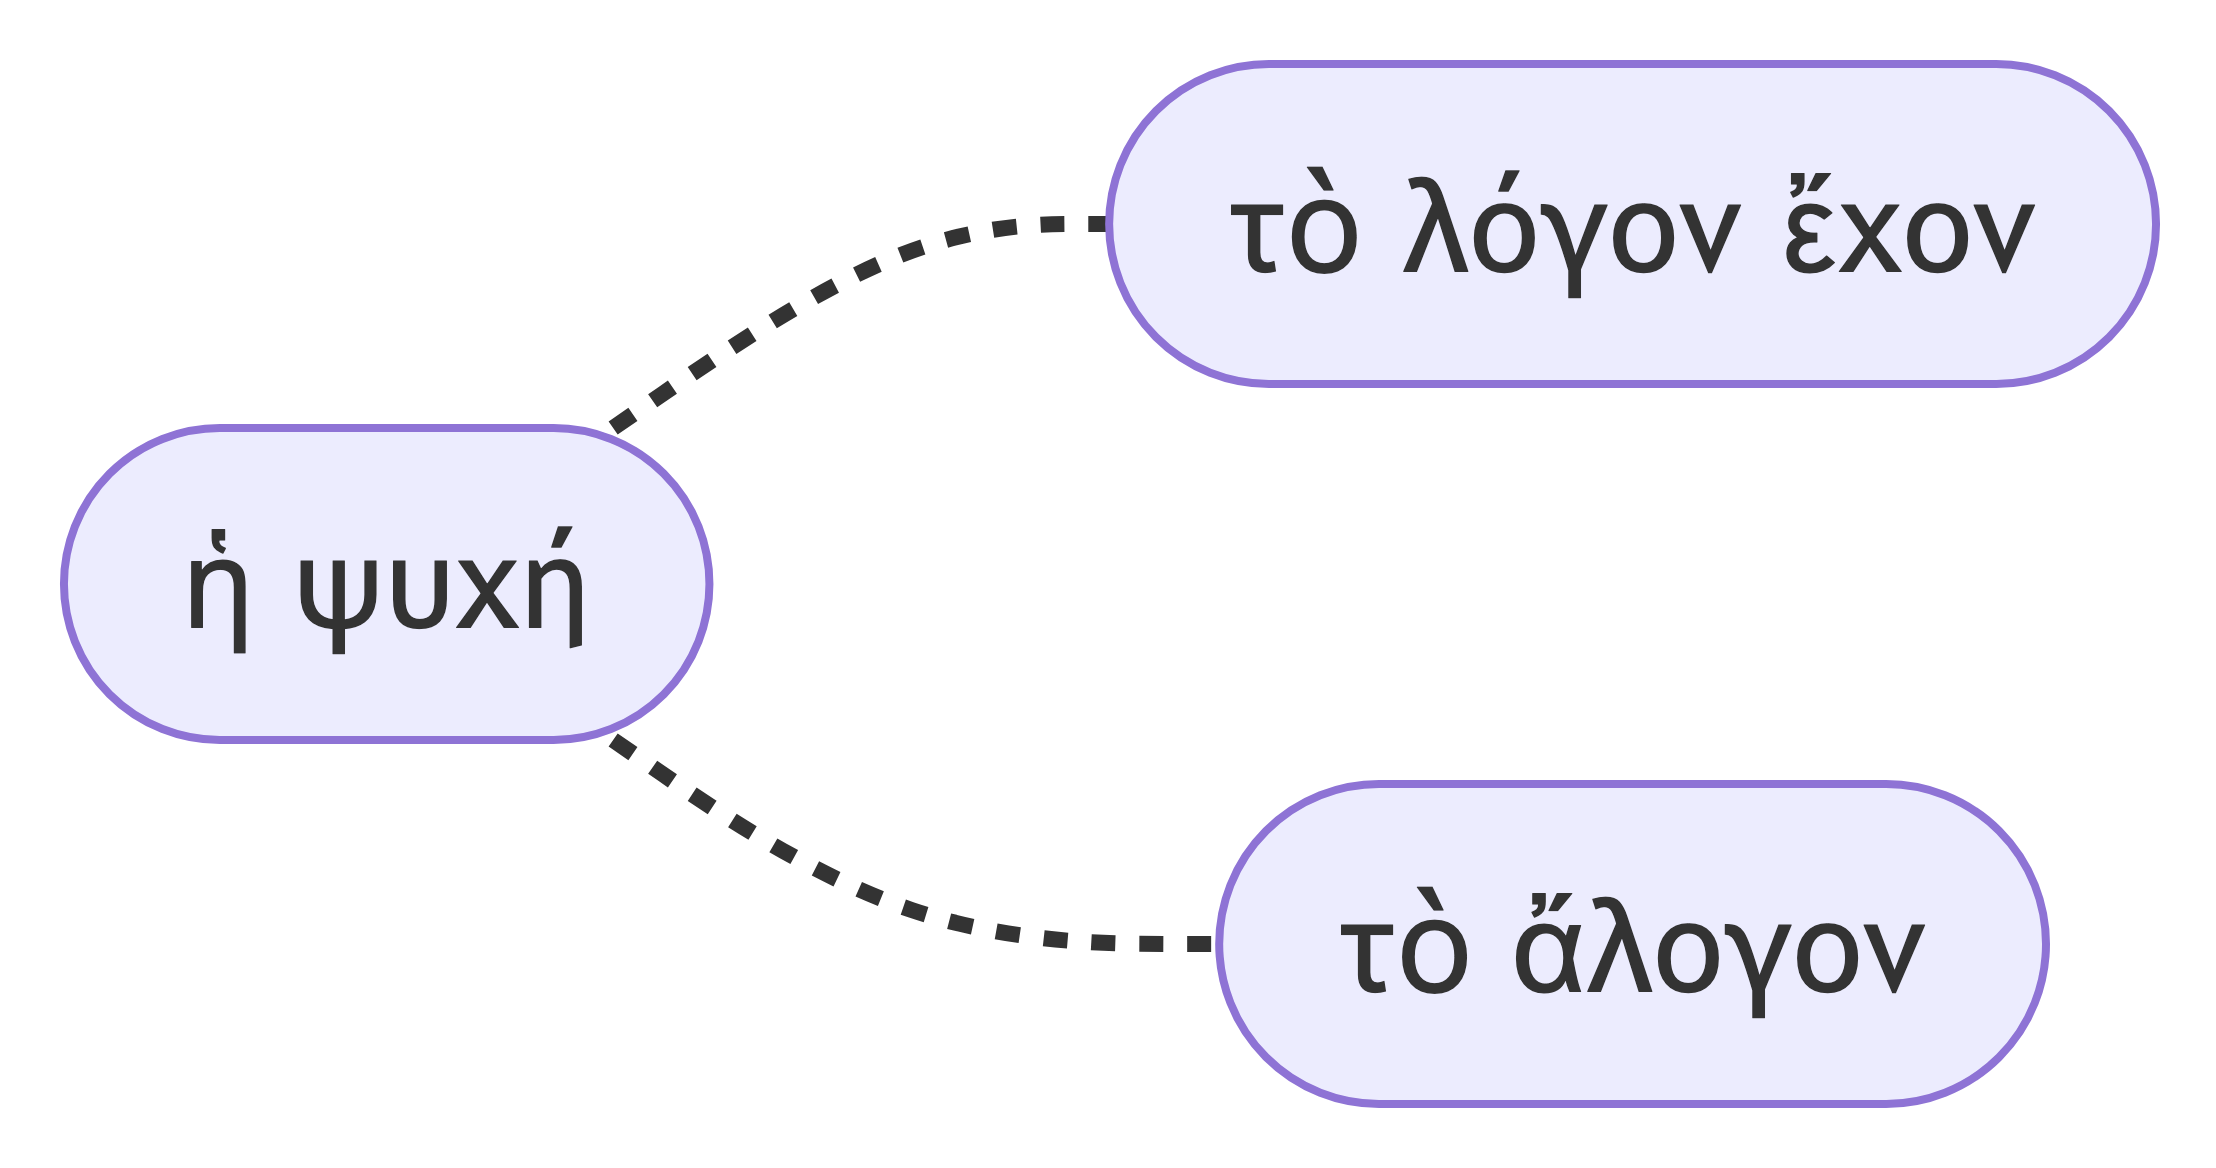
\includegraphics[width=2.89in,height=1.52in]{export_files/figure-latex/mermaid-figure-2.png}

}

\end{figure}

}

\caption{\label{fig-scriv182}ἡ~ψυχή}

\end{figure}

\begin{equation}\protect\hypertarget{eq-scriv182}{}{t' = \frac{t - \dfrac{v}{c^{2}}x}{\sqrt{1 - \dfrac{v^{2}}{c^{2}}}}}\label{eq-scriv182}\end{equation}

\begin{codelisting}

\caption{Ruby code block}

\hypertarget{lst-scriv182}{%
\label{lst-scriv182}}%
\begin{Shaded}
\begin{Highlighting}[numbers=left,,]
\FunctionTok{puts} \StringTok{"Quarto rocks"}
\end{Highlighting}
\end{Shaded}

\end{codelisting}

\hypertarget{tbl-scriv182}{}
\begin{longtable}[]{@{}cc@{}}
\toprule\noalign{}
Markdown Source & Output \\
\midrule\noalign{}
\endfirsthead
\toprule\noalign{}
Markdown Source & Output \\
\midrule\noalign{}
\endhead
\bottomrule\noalign{}
\endlastfoot
\texttt{{[}@DA{]}\{.title\}} & \emph{De Anima} \\
\texttt{{[}@DABiehl1896\ {]}\{.editor\}} & Biehl \\
\texttt{{[}@DABiehl1896{]}\{.issued\}} & 1896 \\
\caption{\label{tbl-scriv182}Table sample}\tabularnewline
\end{longtable}

And see also
\protect\hypertarget{cite_57}{}{\label{cite_57}Equation~\ref{eq-scriv183}},
\protect\hypertarget{cite_58}{}{\label{cite_58}Table~\ref{tbl-scriv184}}.\\
\begin{equation}\protect\hypertarget{eq-scriv183}{}{Equation content
}\label{eq-scriv183}\end{equation}

\hypertarget{tbl-scriv184}{}
\begin{longtable}[]{@{}lll@{}}
\toprule\noalign{}
1 & 2 & 3 \\
\midrule\noalign{}
\endfirsthead
\toprule\noalign{}
1 & 2 & 3 \\
\midrule\noalign{}
\endhead
\bottomrule\noalign{}
\endlastfoot
4 & 5 & 6 \\
\caption{\label{tbl-scriv184}The caption}\tabularnewline
\end{longtable}

\hypertarget{sec-scriv185}{%
\section{CiteTools Integration}\label{sec-scriv185}}

\protect\hypertarget{scriv185}{}{}

\protect\hypertarget{scriv186}{}{} \textsc{1. New} \textbf{Section
Layout} \& \textbf{Section Type} provide support for the multiple
bibliographies Lua Filter.

Choose the Multibib section type, fill the \texttt{Value} custom
meta-data field with the name of your bibliography file (the file
\texttt{ID}, in some cases) and you're set! Do this with as many
bibliographies as you want. The sections will be named after the last
heading element, that is, the binder item whence it originated, as it
happens with all other chapters of the text.

\begin{tcolorbox}[enhanced jigsaw, colbacktitle=quarto-callout-note-color!10!white, leftrule=.75mm, breakable, bottomrule=.15mm, coltitle=black, colback=white, rightrule=.15mm, left=2mm, opacitybacktitle=0.6, opacityback=0, toptitle=1mm, titlerule=0mm, title=\textcolor{quarto-callout-note-color}{\faInfo}\hspace{0.5em}{Note}, arc=.35mm, colframe=quarto-callout-note-color-frame, toprule=.15mm, bottomtitle=1mm]

You can also point Quarto and Pandoc to the bibliography file using
relative paths, full paths and URLs.

\begin{itemize}
\tightlist
\item
  \texttt{my\_file.bib}
\item
  \texttt{/Users/username/bibliography/my\_file.bib}
\item
  \texttt{https://raw.githubusercontent.com/.../arist.bib}
\end{itemize}

\end{tcolorbox}

See the backmatter for examples.

\textsc{2. New} \textbf{Section Type} \& \textbf{Custom Metadata Field}
can be used to override the depth of the current binder item placing the
desired number of hashes in the corresponding metadata field (Depth)
with no space at the end, as in \#\#\#\emph{,} and then selecting the
Depth + Header section type.

\hypertarget{sec-scriv187}{%
\subsection{Cite Field}\label{sec-scriv187}}

\protect\hypertarget{scriv187}{}{}

\marginnote{\begin{footnotesize}

The works of \texttt{{[}@AristOp{]}\{.author\}} were first edited by
\texttt{{[}@AristOp{]}\{.editor\}} in
\texttt{{[}@AristOp{]}\{.issued\}}.

\end{footnotesize}}

\protect\hypertarget{scriv189}{}{} \textsc{New} \textbf{Styles} provide
support for the cite field Lua Filter, which can be used to cite
arbitrary fields of the references.

The works of Aristotelis were first edited by Bekker in 1834. Lorem
ipsum dolor sit amet, consectetur adipisicing elit, sed do eiusmod
tempor incididunt ut labore et dolore magna aliqua. Ut enim ad minim
veniam, quis nostrud exercitation ullamco laboris nisi ut aliquip ex ea
commodo consequat. Duis aute irure dolor in reprehenderit in voluptate
velit esse cillum dolore eu fugiat nulla pariatur. Excepteur sint
occaecat cupidatat non proident, sunt in culpa qui officia deserunt
mollit anim id est laborum.

\marginnote{\begin{footnotesize}

Later, the \texttt{{[}@DA{]}\{.title\}}
(\texttt{{[}@DA{]}\{.title-short\}}) was edited by
\texttt{{[}@DABiehl1896{]}\{.editor\}} in
\texttt{{[}@DABiehl1896{]}\{.issued\}} (reprinted in
\texttt{{[}@DATheiler{]}\{.translator\}\textquotesingle{}s}
\texttt{{[}@DATheiler{]}\{.issued\}} translation)

\end{footnotesize}}

\protect\hypertarget{scriv191}{}{} Later, the \emph{De Anima} was edited
by Biehl in 1896 (reprinted in
{\protect\hypertarget{cite_59}{}{\label{cite_59}THEILER \& SEIDL
\protect\hyperlink{ref-DATheiler}{1995}}}'s 1995 translation). Lorem
ipsum dolor sit amet, consectetur adipisicing elit, sed do eiusmod
tempor incididunt ut labore et dolore magna aliqua. Ut enim ad minim
veniam, quis nostrud exercitation ullamco laboris nisi ut aliquip ex ea
commodo consequat. Duis aute irure dolor in reprehenderit in voluptate
velit esse cillum dolore eu fugiat nulla pariatur. Excepteur sint
occaecat cupidatat non proident, sunt in culpa qui officia deserunt
mollit anim id est laborum.

You can set link-fields to false to avoid undesired linking when citing
specific fields.

\hypertarget{tbl-scriv192}{}
\begin{longtable}[]{@{}cc@{}}
\toprule\noalign{}
Markdown Source & Output \\
\midrule\noalign{}
\endfirsthead
\toprule\noalign{}
Markdown Source & Output \\
\midrule\noalign{}
\endhead
\bottomrule\noalign{}
\endlastfoot
\texttt{{[}@AristOp{]}\{.author\}} & Aristotelis \\
\texttt{{[}@AristOp{]}\{.editor\}} & Bekker \\
\texttt{{[}@AristOp}{]}\{.issued\} & 1834 \\
\texttt{{[}@DA{]}\{.title\}} & \emph{De Anima} \\
\texttt{{[}@DABiehl1896\ {]}\{.editor\}} & Biehl \\
\texttt{{[}@DABiehl1896{]}\{.issued\}} & 1896 \\
\texttt{{[}@DATheiler{]}\{.translator\}} &
{\protect\hypertarget{cite_60}{}{\label{cite_60}THEILER \& SEIDL
\protect\hyperlink{ref-DATheiler}{1995}}} \\
\texttt{{[}@DATheiler{]}\{.issued\}} & 1995 \\
\caption{\label{tbl-scriv192}Simple example of how we are using styles
to create the correct markup}\tabularnewline
\end{longtable}

\textsc{4. Added} the prefix
\texttt{{[}{]}\{\#scriv\textbackslash{}\textless{}\$linkID\textgreater{}\}}
to some \textbf{Section Layouts}.

This allows us to create links to \protect\hyperlink{scriv193}{text
sections that do not have a Header element}.

\protect\hypertarget{scriv194}{}{} Belive it or not, Scrivener can be an
interesting place to keep parts of your code. We can use the document
bookmarks to leave behind an array of possibilities in case we need to
revise something. We can easily copy and paste code stored on Quarto's
Github repository to compare using Scrivener's superior text matching
tool! (My favorite comparison tool is placing the text in different
documents and using \enquote{matching text} in the Bookmark tab of the
right-side inspector in Scrivener.)

\begin{figure}

{\centering 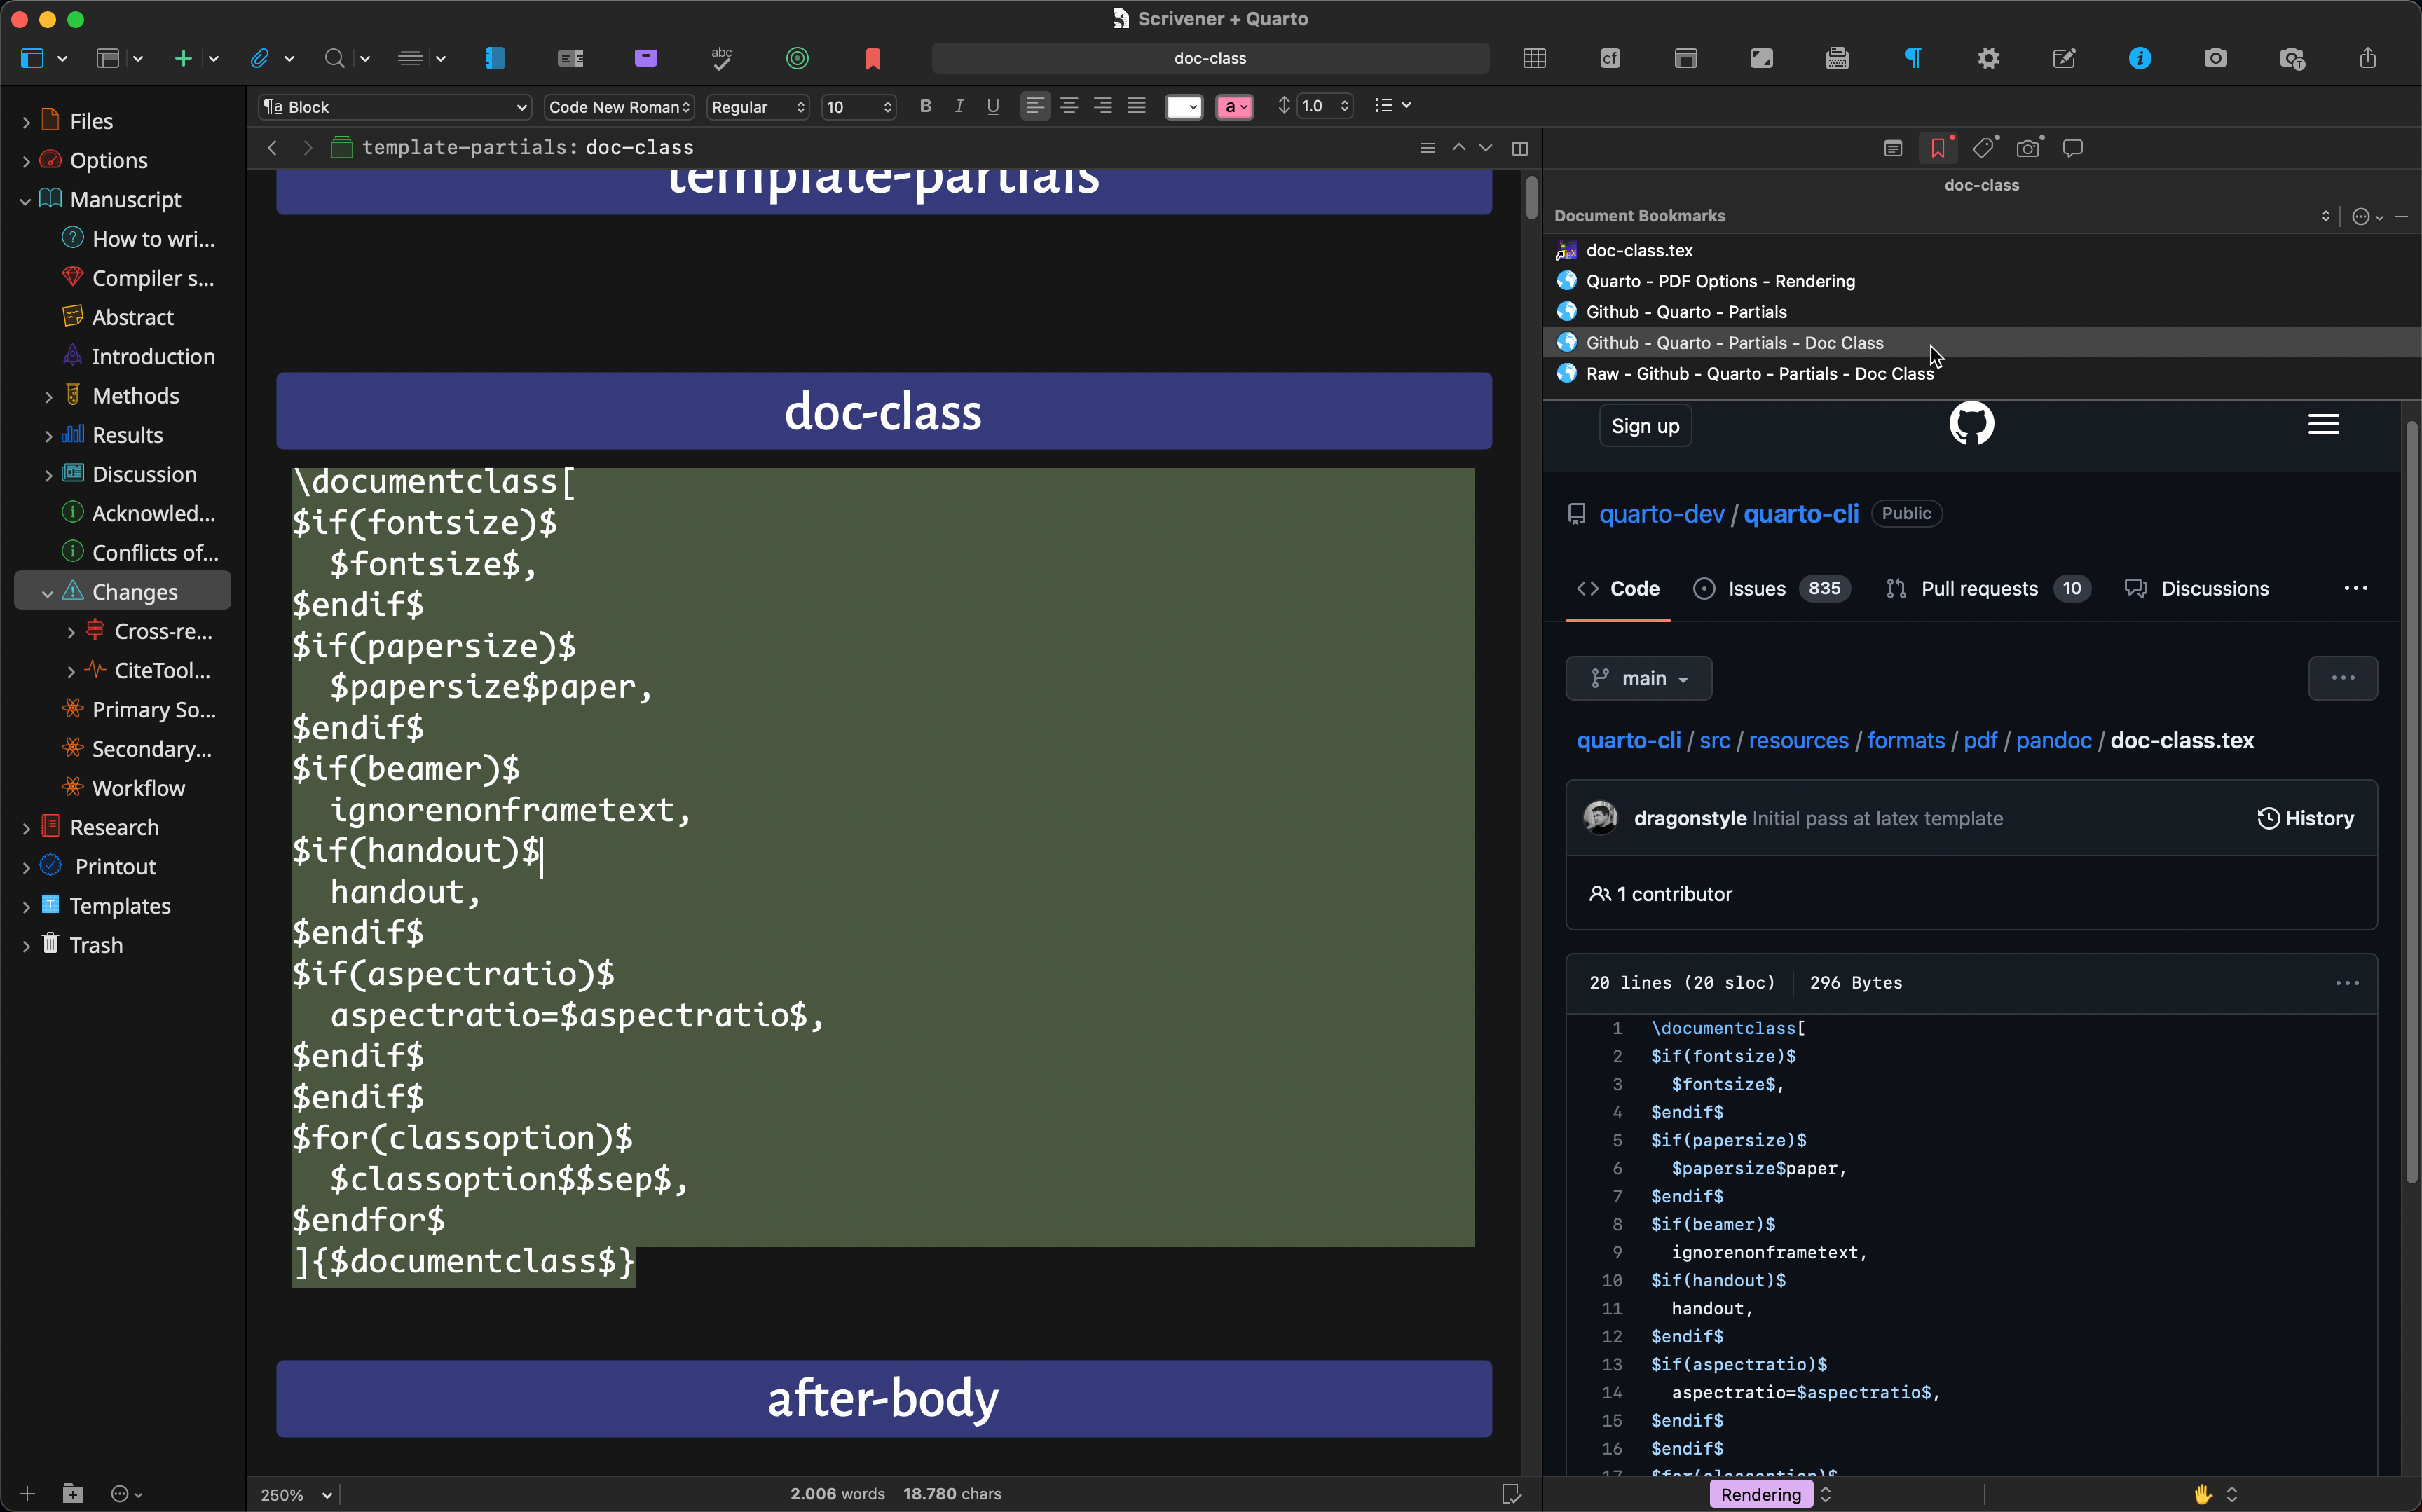
\includegraphics[width=5.77083in,height=3.60417in]{scrivenerwithcode.png}

}

\caption{\label{fig-scriv194}Revising code in Scrivener can be just as
pleasant}

\end{figure}

\protect\hypertarget{scriv195}{}{}

We can also create interesting possibilities to customize and further
control the conversion process, by including in our project the default
Pandoc Latex Templates. Customize any line of the whole code. Or not,
maybe just leave it there and take a look every once in a while at what
is going on at the Quarto repository. The template will work either way.

\begin{figure*}

{\centering 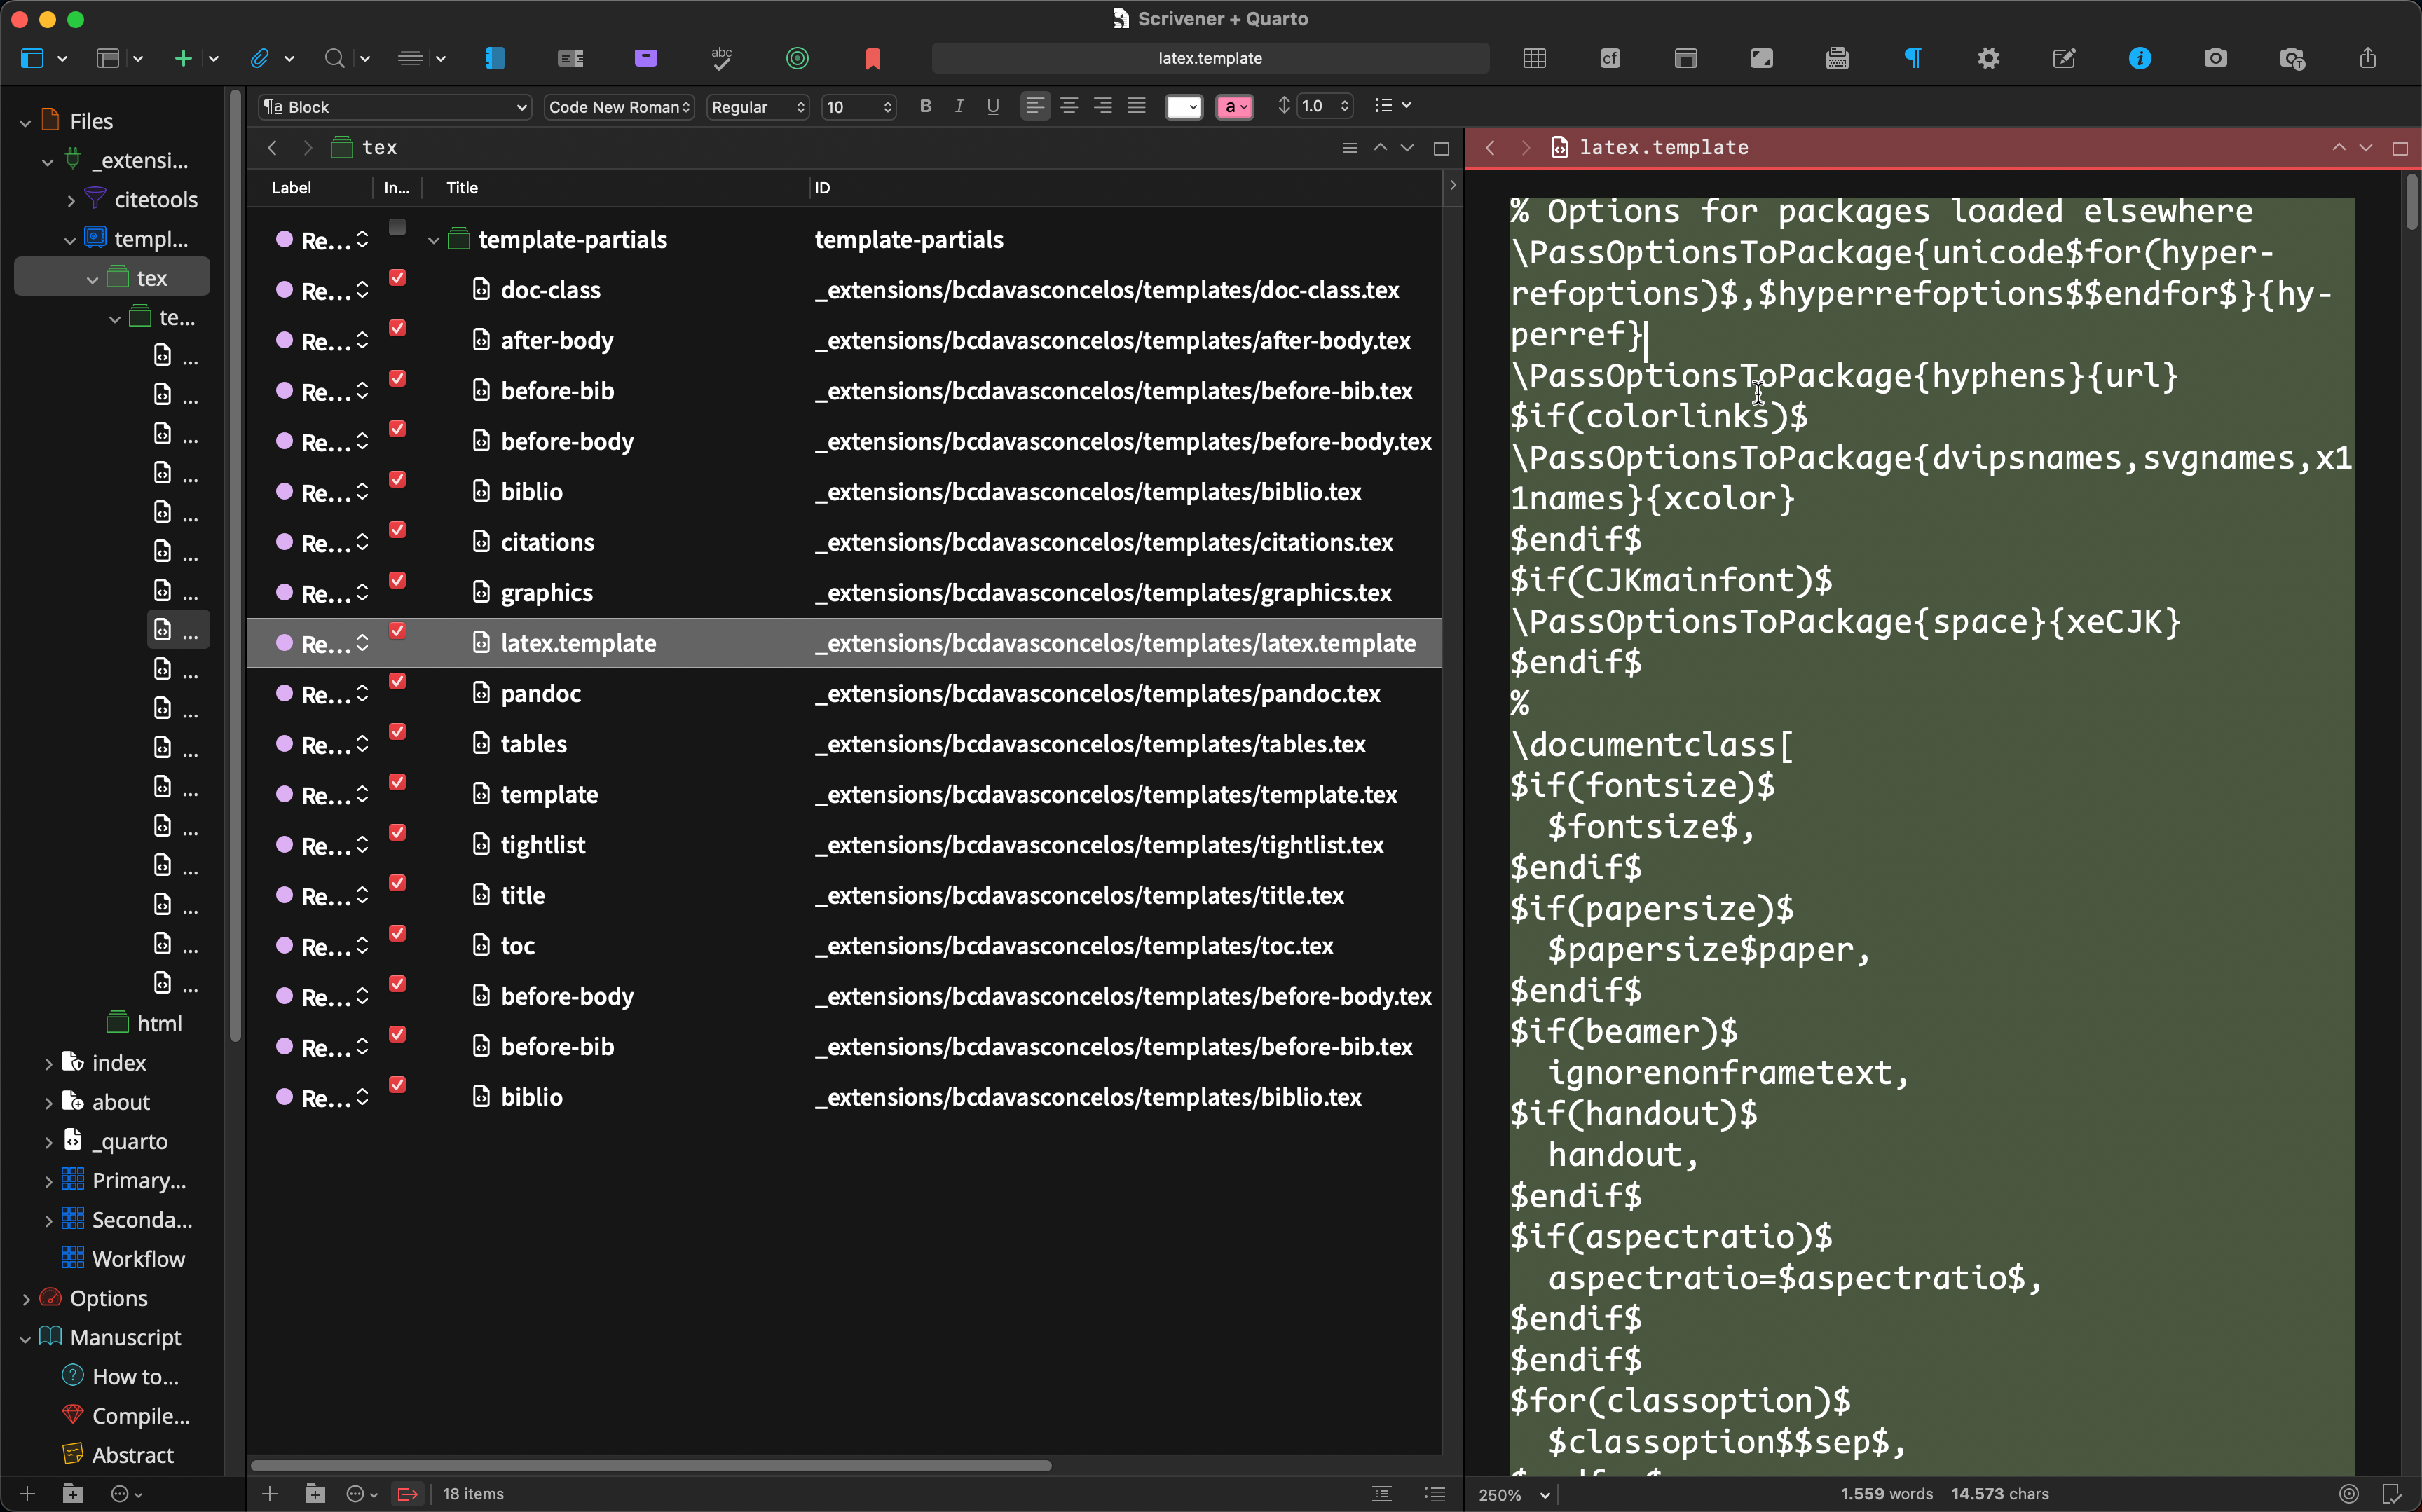
\includegraphics[width=5.69792in,height=3.5625in]{pandocquartolatextemplate.png}

}

\caption{\label{fig-scriv195}Students finishing their MDs or PhDs will
certainly appreciate the possibility of adding your own latex
customizations, which can also be done by including the code within
certain fields, such as before-body.}

\end{figure*}

\begin{tcolorbox}[enhanced jigsaw, colbacktitle=quarto-callout-important-color!10!white, leftrule=.75mm, breakable, bottomrule=.15mm, coltitle=black, colback=white, rightrule=.15mm, left=2mm, opacitybacktitle=0.6, opacityback=0, toptitle=1mm, titlerule=0mm, title=\textcolor{quarto-callout-important-color}{\faExclamation}\hspace{0.5em}{Important}, arc=.35mm, colframe=quarto-callout-important-color-frame, toprule=.15mm, bottomtitle=1mm]

If you are having problems with performance, then you should try to
delete the custom icons we are using. I recommend deleting all to see if
that makes a difference or not on how Scrivener is behaving.

\end{tcolorbox}

\begin{tcolorbox}[enhanced jigsaw, colbacktitle=quarto-callout-tip-color!10!white, leftrule=.75mm, breakable, bottomrule=.15mm, coltitle=black, colback=white, rightrule=.15mm, left=2mm, opacitybacktitle=0.6, opacityback=0, toptitle=1mm, titlerule=0mm, title=\textcolor{quarto-callout-tip-color}{\faLightbulb}\hspace{0.5em}{Tip}, arc=.35mm, colframe=quarto-callout-tip-color-frame, toprule=.15mm, bottomtitle=1mm]

Right click on any Binder item.
\texttt{Change\ Icon\ \textgreater{}\ Manage\ Custom\ Icons...}

\end{tcolorbox}

\hypertarget{sec-scriv198}{%
\chapter{Primary Sources}\label{sec-scriv198}}

\hypertarget{refs_scriv198}{}
\begin{CSLReferences}{0}{1}
\leavevmode\vadjust pre{\hypertarget{ref-AristOp}{}}%
ARISTOTELIS. \emph{Aristotelis Opera}. Ed.: I. Bekker. Berlin: Reimer,
1834. {[}\Acrobatmenu{GoBack}{$\hookleftarrow$}{]}

\leavevmode\vadjust pre{\hypertarget{ref-DA}{}}%
ARISTOTELIS. {`De Anima'}. In: BEKKER, I. (Ed.). \emph{Aristotelis
Opera}. Berlin: Reimer, 1834.
{[}\Acrobatmenu{GoBack}{$\hookleftarrow$}{]}

\end{CSLReferences}

\hypertarget{sec-scriv199}{%
\chapter{Secondary Sources}\label{sec-scriv199}}

\hypertarget{refs_scriv199}{}
\begin{CSLReferences}{0}{1}
\leavevmode\vadjust pre{\hypertarget{ref-DABiehl1896}{}}%
ARISTOTELIS. \emph{De Anima}. Ed.: W. Biehl. Leipzig: Teubner, 1896.
{[}\Acrobatmenu{GoBack}{$\hookleftarrow$}{]}

\leavevmode\vadjust pre{\hypertarget{ref-DATheiler}{}}%
ARISTOTELIS. \emph{De Anima}. Eds.: W. Theiler \& H. Seidl. Harmburg:
Felix Meiner, 1995. {[}\Acrobatmenu{GoBack}{$\hookleftarrow$},
\protect\hyperlink{cite_59}{\pageref{cite_59}},
\protect\hyperlink{cite_60}{\pageref{cite_60}}{]}

\end{CSLReferences}

\hypertarget{sec-scriv200}{%
\chapter{Workflow}\label{sec-scriv200}}

\hypertarget{refs_scriv200}{}
\begin{CSLReferences}{0}{1}
\leavevmode\vadjust pre{\hypertarget{ref-barrett2015}{}}%
BARRETT, L.; SIMMONS, W.
\href{https://doi.org/10.1038/nrn3950}{Interoceptive predictions in the
brain.} \emph{Nature Reviews Neuroscience}, v. 16, n. 7, p. 419--429,
2015. {[}\Acrobatmenu{GoBack}{$\hookleftarrow$},
\protect\hyperlink{cite_2}{\pageref{cite_2}},
\protect\hyperlink{cite_5}{\pageref{cite_5}},
\protect\hyperlink{cite_6}{\pageref{cite_6}},
\protect\hyperlink{cite_7}{\pageref{cite_7}},
\protect\hyperlink{cite_36}{\pageref{cite_36}}{]}

\leavevmode\vadjust pre{\hypertarget{ref-copenhaver2014}{}}%
COPENHAVER, R. \href{}{Berkeley on the language of nature and the
objects of vision}. \emph{Res Philosophica}, v. 91, n. 1, p. 29--46,
2014. {[}\Acrobatmenu{GoBack}{$\hookleftarrow$},
\protect\hyperlink{cite_5}{\pageref{cite_5}}{]}

\leavevmode\vadjust pre{\hypertarget{ref-crivellato2007}{}}%
CRIVELLATO, E.; RIBATTI, D.
\href{https://doi.org/10.1016/j.brainresbull.2006.09.020}{Soul, mind,
brain: Greek philosophy and the birth of neuroscience}. \emph{Brain
Research Bulletin}, v. 71, n. 4, p. 327--336, 2007.
{[}\Acrobatmenu{GoBack}{$\hookleftarrow$},
\protect\hyperlink{cite_1}{\pageref{cite_1}},
\protect\hyperlink{cite_2}{\pageref{cite_2}},
\protect\hyperlink{cite_3}{\pageref{cite_3}},
\protect\hyperlink{cite_7}{\pageref{cite_7}},
\protect\hyperlink{cite_26}{\pageref{cite_26}},
\protect\hyperlink{cite_36}{\pageref{cite_36}}{]}

\leavevmode\vadjust pre{\hypertarget{ref-hoffman2014}{}}%
HOFFMAN, D. D.; PRAKASH, C.
\href{https://doi.org/10.3389/fpsyg.2014.00577}{Objects of
consciousness}. \emph{Frontiers in Psychology}, v. 5, p. 577, 2014.
{[}\Acrobatmenu{GoBack}{$\hookleftarrow$},
\protect\hyperlink{cite_5}{\pageref{cite_5}}{]}

\leavevmode\vadjust pre{\hypertarget{ref-siegel2015}{}}%
SIEGEL, S.; SILINS, N. {`The epistemology of perception'}. In: MATTHEN,
M. (Ed.). \emph{Oxford handbook of philosophy of perception}. Oxford
University Press, 2015. p. 1--48.
{[}\Acrobatmenu{GoBack}{$\hookleftarrow$},
\protect\hyperlink{cite_5}{\pageref{cite_5}},
\protect\hyperlink{cite_12}{\pageref{cite_12}},
\protect\hyperlink{cite_13}{\pageref{cite_13}},
\protect\hyperlink{cite_17}{\pageref{cite_17}},
\protect\hyperlink{cite_21}{\pageref{cite_21}},
\protect\hyperlink{cite_27}{\pageref{cite_27}},
\protect\hyperlink{cite_32}{\pageref{cite_32}},
\protect\hyperlink{cite_33}{\pageref{cite_33}},
\protect\hyperlink{cite_34}{\pageref{cite_34}},
\protect\hyperlink{cite_35}{\pageref{cite_35}},
\protect\hyperlink{cite_36}{\pageref{cite_36}}{]}

\leavevmode\vadjust pre{\hypertarget{ref-simmons2013}{}}%
SIMMONS, A. {`Perception in early modern philosophy'}. In: MATTHEN, M.
(Ed.). \emph{The oxford handbook of philosophy of perception}. Oxford:
Oxford University Press, 2013.
{[}\Acrobatmenu{GoBack}{$\hookleftarrow$},
\protect\hyperlink{cite_5}{\pageref{cite_5}}{]}

\end{CSLReferences}


\backmatter

\end{document}
